\documentclass[12pt]{article}

% per immagini
\usepackage{graphicx}
\usepackage{float}
\usepackage[italian, english]{babel}

% margini pagina
\usepackage[top=1.2in, right = 0.8in, left = 0.8in, bottom=0.8in]{geometry}
\usepackage{fancyhdr}
\pagestyle{fancy}
\fancyhf{}
\lhead{}
\lfoot{}
\rfoot{\thepage}
\renewcommand{\headrulewidth}{0pt}
\renewcommand{\footrulewidth}{0pt}
\setlength{\footskip}{15pt}

% abstract
\usepackage{abstract} % Allows abstract customization
\renewcommand{\abstractnamefont}{\normalfont\bfseries} % Set the "Abstract" text to bold
\renewcommand{\abstracttextfont}{\normalfont\itshape} % Set the abstract itself to small italic text

\usepackage{titling} % Customizing the title section
\setlength{\droptitle}{-3\baselineskip} % Move the title up

% bibliography
\usepackage{csquotes}
\usepackage[sorting=none]{biblatex}
\addbibresource{biblio.bib}
\usepackage[pdfusetitle, colorlinks=true,linktoc=page,allcolors=blue]{hyperref}

% per tabella
\usepackage{longtable,tabularx}
\newcolumntype{L}[1]{>{\raggedright\let\newline\\\arraybackslash\hspace{0pt}}m{#1}}
\newcolumntype{C}[1]{>{\centering\let\newline\\\arraybackslash\hspace{0pt}}m{#1}}
%\renewcommand{\arraystretch}{1.5}
%\renewcommand{\familydefault}{\sfdefault}

% per json
\usepackage{xcolor}
\usepackage{listings}

\newcommand\JSONnumbervaluestyle{\color{blue}}
\newcommand\JSONstringvaluestyle{\color{red}}

% switch used as state variable
\newif\ifcolonfoundonthisline

\makeatletter

\lstdefinestyle{json}
{
  showstringspaces    = false,
  keywords            = {false,true},
  alsoletter          = 0123456789.,
  morestring          = [s]{"}{"},
  stringstyle         = \ifcolonfoundonthisline\JSONstringvaluestyle\fi,
  MoreSelectCharTable =%
    \lst@DefSaveDef{`:}\colon@json{\processColon@json},
  basicstyle          = \ttfamily,
  keywordstyle        = \ttfamily\bfseries,
}

% flip the switch if a colon is found in Pmode
\newcommand\processColon@json{%
  \colon@json%
  \ifnum\lst@mode=\lst@Pmode%
    \global\colonfoundonthislinetrue%
  \fi
}

\lst@AddToHook{Output}{%
  \ifcolonfoundonthisline%
    \ifnum\lst@mode=\lst@Pmode%
      \def\lst@thestyle{\JSONnumbervaluestyle}%
    \fi
  \fi
  %override by keyword style if a keyword is detected!
  \lsthk@DetectKeywords% 
}

% reset the switch at the end of line
\lst@AddToHook{EOL}%
  {\global\colonfoundonthislinefalse}

%%%% documento 
\title{\textbf{Airline On-Time Performance}}

\author{
Riccardo Confalonieri \\ CdLM Data Science\\
                matr. 830404 
\and
Rebecca Picarelli \\  CdLM Data Science\\
                matr. 834286 
\and
Silvia Ranieri\\  CdLM Data Science\\
                matr. 878067
}              

\date{Progetto di Data Management \& Data Visualization\\Appello di Giugno 2021 }

% definisco l'abstract
\renewcommand{\maketitlehookd}{%
\vspace{50pt}
\begin{abstract}
\noindent Negli Stati Uniti, a causa delle dimensioni del territorio, è noto che gli spostamenti aerei siano molto frequenti e talvolta proprio necessari. Di conseguenza, potrebbe risultare interessante analizzare a livello quantitativo questo fenomeno, prestando attenzione soprattutto ai ritardi registrati per i singoli voli, per capire, magari, quali possano essere i periodi e/o le compagnie migliori per viaggiare. Dunque, grazie ai dati fonti dal sito del Dipartimento dei trasporti degli Stati Uniti d’America e in particolare dall’agenzia governativa ``Bureau of Transportation Statistics'' (BTS), è stato possibile scaricare i dati relativi ai voli statunitensi interni per gli anni 2018 e 2019, che sono stati poi integrati con informazioni provenienti da altre fonti. Relativamente a quest’ultime, sulla piattaforma Kaggle è stato possibile scaricare dataset contenenti informazioni aggiuntive per quanto riguarda le compagnie aeree e gli aeroporti. Infine, dal sito del ``Airports Council International - North America'' (ACI) sono stati reperiti dei dati inerenti al numero di passeggeri per alcuni dei principali aeroporti in diversi anni.
Inoltre, grazie a linguaggio Python e a MongoDB, ovvero un DataBase Management System di tipo non relazionale orientato ai documenti, è stato possibile creare un’architettura adatta a gestire grandi volumi di dati, ossia una delle “V” caratteristiche dei big data, congiuntamente all’aspetto della varietà.
Infine, nella seconda parte del lavoro sono riportate alcune delle infografiche, realizzate sfruttando il software Tableau Desktop, con l'obiettivo di rappresentare alcune possibili informazioni non chiaramente individuabili da una semplice lettura dei dati.
\end{abstract}
\vspace{50pt}
\newpage
}

\begin{document}

\maketitle
\thispagestyle{fancy}

\selectlanguage{italian}
\hypersetup{linkcolor=black}
\tableofcontents

\newpage
\part{Data Management}
\section{Introduzione}
Negli Stati Uniti, considerando l’ultimo ventennio circa, si è notato un trend in costante crescita per quanto riguarda sia il profitto ricavato dalle compagnie aeree sia in termini di movimentazione dei passeggeri e del numero totale di voli, internazionali e locali. Questo andamento crescente si è intensificato soprattutto a partire dal 2014 ma anche nel biennio 2018-2019, ovvero quello di nostro interesse, si è verificato un +4\% sul totale dei voli e ben un +25\%, corrispondente a 14.8 miliardi di dollari, in termini di fatturato.\\
Tali cifre in continua crescita ci hanno spinto a raccogliere i dati sui voli USA 2018 e 2019 per analizzare in particolar modo i ritardi dei voli e dunque trovare se esiste un mese e/o una compagnia migliore per volare.

\section{Ricerca dei dati}
Individuato il problema da analizzare per il progetto ci siamo concentrati sulla ricerca dei dati necessari. Le informazioni di base per lo scopo preposto erano quelle riguardati i voli statunitensi, disponibili sul sito governativo ``Bureau of Transportation Statistics''\cite{BTS}. Una volta individuata la fonte principale dei nostri dati ci siamo concentrati su come arricchire i dati a disposizione per riuscire a creare un'unica informazione il più completa possibile. Nei paragrafi successivi sono descritti i passaggi effettuati per ottenere i dati.

\subsection{Dati sui voli USA}
Per scaricare le informazioni sui voli ci si è serviti di Python e del tool open source Selenium che ha permesso, dopo aver individuato direttamente sul sito governativo del BTS\cite{BTS} le 32 variabili rilevanti ai fini dell’analisi, di automatizzare il procedimento di scraping dei dati di interesse. L’automatizzazione del download dei dati garantisce sia di eliminare eventuali errori sulla scelta manuale di mese in mese delle variabili sia di ottenere in automatico il file .csv che veniva scaricato dal sito in formato zippato risparmiando così tempo e operazioni manuali. Nella pagina seguente si riportano le variabili ottenute, i campi contrassegnati con * possono presentare valori nulli:

% change margin for fix table
\newgeometry{top=1in, right = 0.8in, left = 0.8in, bottom=0.8in}
% change arraystretch for this table
\renewcommand{\arraystretch}{1.5}
\begin{longtable}{ L{6.2cm} L{10.3cm} }
    
    \hline
    \textbf{Variabili} & \textbf{Descrizione} \\\hline \endhead
    \hline
        \textbf{Data}\\
        1. Year & Anno del volo\\ 
        2. Month & Mese del volo \\
        3. DayOfmonth& Giorno del mese del volo\\
        4. DayOfweek& Giorno della settimana del volo\\
    \hline
        \textbf{Compagnia aerea}\\
        5. IATA\_CODE\_Reporting\_Airline& Codice IATA identificativo della compagnia aerea.\\
    \hline    
        \textbf{Origine e destinazione}\\
        6. Origin&Codice IATA identificativo dell'aeroporto di partenza.\\
        7. OriginCityName&Città di partenza e abbreviazione USPS del nome dello stato.\\
        8. OriginStateName&Nome per esteso dello stato di partenza.\\
        9. Dest&Codice IATA identificativo dell'aeroporto di arrivo.\\
        10. DestCityName&Città di arrivo e abbreviazione USPS del nome dello stato.\\
        11. DestStateName&Nome per esteso dello stato di arrivo.\\
    \hline    
        \textbf{Performance sulla partenza}\\
        12. CRSDepTime&Orario di partenza programmato  (formato hhmm).\\
        13. DepTime*&Orario di partenza effettivo (formato hhmm).\\
        14. DepDelay*&Differenza in minuti tra l'orario di partenza previsto e quello effettivo. Le partenze anticipate mostrano numeri negativi. \\
        15. DepartureDelayGroups*&Intervalli di ritardo partenza, ogni 15 minuti da $<$-15 a $>$180. \\
    \hline
        \textbf{Performance sull'arrivo}\\
        16. CRSArrTime& Orario di arrivo programmato (formato hhmm).\\
        17. ArrTime*&Orario di arrivo effettivo (formato hhmm).\\
        18. ArrDelay*&Differenza in minuti tra l'orario di arrivo previsto e quello effettivo. Gli arrivi anticipati mostrano numeri negativi. \\
        19. ArrivalDelayGroups*&Intervalli di ritardo in arrivo, ogni 15 minuti da $<$-15 a $>$180.\\
    \hline
        \textbf{Annullamenti e deviazioni}\\
        20. Cancelled&Indica se il volo è stato cancellato (1 = true).\\
        21. CancellationCode*&Specifica la ragione di cancellazione.\\
        22. Diverted&Indica se il volo è stato dirottato su un altro aeroporto (1 = true).\\
    \hline
        \textbf{Informazioni sul volo}\\
        23. CRSElapsedTime&Durata prevista del volo.\\
        24. ActualElapsedTime*&Durata effettiva del volo.\\
        25. AirTime*&Tempo in volo.\\ 
        26. Distance&Distanza tra gli aeroporti in miglia.\\
        27. DistanceGroup&Intervalli di distanza, raggruppati ogni 250 miglia.\\
    \hline
        \textbf{Cause del ritardo}\\
        28. CarrierDelay*&Ritardo dovuto alla manutenzione, all’equipaggio, alla pulizia della cabina, all’imbarco dei bagaglio o alla benzina che può richiedere fino a 2h su grossi veivoli.\\
        29. WeatherDelay*&Ritardo legato al meteo.\\
        30. NASDelay*&National Aviation System Delay, ritardi legati al traffico aereo e/o operazioni aereoportuali\\ 
        31. SecurityDelay*&Ritardi dovuti a situazioni critiche che  richiedono  evacuazioni,  violazioni della sicurezza a bordo o problemi nelle aree di screening.\\
        32. LateAircraftDelay*&Ritardo dell'aereo, si verifica spesso su voli sequenziali e causa reazioni e ritardi a catena.\\
\end{longtable}

\noindent Analizzando la struttura dei dati si può notare che le cause del ritardo vengono espresse soltanto per i ritardi superiori ai 15 minuti, e inoltre nel caso di volo cancellato o dirottato tutti i campi riportanti performance  e tempistiche effettive risultano nulli.
\restoregeometry

\subsection{Dati sulle compagnie aeree}
Ottenute le informazioni di base ci siamo concentrati sulla ricerca di altre fonti di dati che permettessero di arricchire le informazioni a nostra disposizione. Dato che dal sito BTS è possibile scaricare soltanto il codice IATA della compagnia aerea, codice poco conosciuto ed utilizzato in quanto normalmente le persone utilizzano il nome completo della compagnia, si è optato per cercare un dataset che permettesse di aggiungere proprio quest'ultima informazione alla nostra base di dati.\\
In questo caso l'informazione era reperibile in numerosi dataset online, in particolare su Kaggle\cite{kaggleAirlines}, sito dal quale abbiamo scaricato il dataset in formato tabellare con la seguente struttura:
\begin{verbatim}
    Airline ID,Name,Alias,IATA,ICAO,Callsign,Country,Active
\end{verbatim}
In particolare, nel nostro caso specifico, ci siamo concentrati sui campi ``IATA'' e ``Name''. Il primo ha permesso di fare il match con la variabile ``IATA\_CODE\_Reporting\_Airline'' precedentemente scaricata, mentre il secondo campo contiene proprio l'informazione da noi ricercata.

\subsection{Dati sugli aeroporti}
Come per le compagnie aeree, anche i dati direttamente ottenibili sugli aeroporti erano abbastanza esigui. Sfruttando nuovamente un dataset reperibile su Kaggle\cite{kaggleAirports} abbiamo integrato le informazioni di base disponibili aggiungendone di più dettagliate. In questo caso il formato tabellare scaricato avente la seguente struttura:
\begin{verbatim}
    ident,type,name,elevation_ft,continent,iso_country,iso_region,municipality,
    gps_code,iata_code,local_code,coordinates
\end{verbatim}
ci ha permesso di inserire come informazioni il tipo di aeroporto, l'altitudine, il codice ICAO, e le sue coordinate ottenibili rispettivamente dalle variabili ``type'', ``elevation\_ft'', ``gps\_code''  e ``coordinates''. Mentre la variabile ``iata\_code'' è stata utilizzata per effettuare il match con le variabili, sui voli, ``origin'' e ``dest'' precedentemente scaricate.

\subsection{Dati sui passeggeri}
Infine, l'ultima informazione ricercata per l'integrazione riguarda il numero di passeggeri in transito nei vari aeroporti. Questa informazione non era facilmente reperibile in quanto i siti governativi statunitensi tendono a rilasciarla solamente negli anni successivi o a pagamento. Una buona base di dati per l'integrazione è stata però trovata sul sito del ``Airports Council International''\cite{ACI}, dove attraverso una particola URL è stato possibile scaricare i file contenenti il numero totale di passeggeri per gli anni 2018 e 2019 dei primi 50 aeroporti nordamericani, di cui quasi tutti sono statunitensi. Oltre al numero totale di passeggeri il file fornisce anche il ranking mondiale dell'aeroporto e il tasso di crescita del numero di passeggeri rispetto all'anno precedente.\\
In questo caso il file scaricato è in formato .xlsx con la seguente struttura tabellare:
\begin{verbatim}
    World Ranking |	NAM Ranking	 | Country | City/State	| Airport Code | 
    Total Passengers |	% Chg 2019-2018
\end{verbatim}
Questi dati ci hanno permesso di arricchire le informazioni inserendo, per gli aeroporti presenti nel file, il totale dei passeggeri transitati, il rispettivo ranking mondiale e il tasso di crescita sul numero di passeggeri.

\newpage
\section{Gestione dei dati}
Dopo aver individuato e scaricato le sorgenti dati necessarie per il progetto ci siamo concentrati sulla fase d'integrazione dei dati. Analizzando i dati scaricati è risultato evidente che uno degli aspetti critici da considerare era il volume dei dati in quanto considerando solamente i dati sui voli per il biennio 2018-2019, senza alcuna integrazione, si superavano ampiamente i 2GB. Per questa motivazione abbiamo deciso di memorizzare i dati su MongoDB, un database orientato ai documenti json binarizzati (BSON), che permette una buona scalabilità anche di fronte ad alti volumi di dati.\\
Avendo optato per l'utilizzo di MongoDB è stato necessario convertire i dati dal formato csv col quale venivano scaricati al formato json. Durante la conversione abbiamo anche svolto la fase d'integrazione risparmiando così tempo e risorse in quanto i file csv riguardanti i voli, ovvero i più pesanti in termini di volume, venivano letti, integrati con le nuove informazioni e convertiti in un solo passaggio.

\subsection{Scelte implementative}
Prima di iniziare la fase vera e propria di conversione al formato json ed arricchimento dei dati abbiamo analizzato la tipologia di dati a nostra disposizione. I dati scaricati per l'arricchimento risultavano già ottimali, erano infatti presenti alcuni valori null nelle colonne di particolari aeroporti o compagniee aeree che però non erano di nostro interesse. Al contrario per i dati sui voli abbiamo dovuto effettuare diverse scelte dovute alla tipologia di partenza dei dati e allo tipologie offerte per lo storage da MongoDB. In particolare ci siamo soffermati sui seguenti casi:
\begin{enumerate}
    \item I campi data. Nel dataset di partenza la data era suddivisa in campi diversi, in questo caso abbiamo deciso di mantenere i tre campi separati e salvarli su mongo come stringhe separate per due motivazioni: da un lato ha permesso di evitare la conversione del formato prima dell'upload dei dati, dall'altro lato sia per le visualizzazioni che avevamo in mente sia per i match necessari nelle query era più semplice poter gestire ed interrogare singolarmente questi campi. Ad esempio mantenendo questa separazione è molto semplice selezionare un particolare mese senza doversi preoccupare dell'anno e dei giorni specifici.
    \item Il formato dell'ora. In questo caso mongo non offriva un format per l'ora che non includesse la data, quindi come nel caso precedente abbiamo optato per salvarla come intero nel formato hhmm. In questo caso la scelta è dovuta in parte al risparmio di spazio in quanto per inserirla in un formato apposito avremmo dovuto aggiungere ogni volta anche un riferimento alla data, che però sarebbe stato non solo duplicato con i campi data già presenti ma anche tra i diversi campi ora in quanto nel dataset sono presenti le ore di partenza effettiva e prevista e gli stessi due campi anche per l'arrivo. Inoltre questa scelta non preclude la possibilità di effettuare query con un intervallo di ore specifico, essendo campi interi infatti basterà matchare questi campi inserendo il massimo e minimo valore desiderato. \\
    Questa scelta rimane consistente e valida grazie al formato delle 24h utilizzato nel file csv originario che dunque non contiene nessun volo in partenza alle 00:00, inoltre i voli in partenza negli orari notturni sono memorizzati senza zeri davanti dunque un volo in partenza alle 00:30 del mattino ad esempio è salvato nel file csv come 30.
    \item I campi con valori nulli. In questo caso la gestione è stata facilitata per via della scelta di un database NoSQL, dato che una delle caratteristiche principali di questi database è la mancanza di una struttura rigida abbiamo inserito nel file json soltanto i campi contenenti valori validi.
    \item Il totale delle righe. Dato che in media ogni mese dell'anno contiene nel formato csv circa 500mila righe è stato necessario trovare un raggruppamento dei dati più ottimale per evitare di caricare nel database MongoDB oltre 6milioni di documenti per ogni anno d'interesse. Per questo si è deciso di raggruppare i dati oltre che per anno e mese, raggruppamento già fornito in partenza in quanto i dati erano scaricati mese per mese dal sito governativo USA, anche per origine, destinazione del volo e giorno della settimana. Questo raggruppamento risponde anche all'idea di voler trovare un giorno o un periodo migliore per volare e non una specifica data all'interno di un mese. Questo tipo di raggruppamento ci ha permesso di passare da oltre 500mila file json necessari per ogni mese a circa 33mila file per mese, in ogni file infatti sono presenti più voli.
\end{enumerate}
Una volta considerate tutte queste necessità abbiamo iniziato a costruire la struttura generale che desideravamo ottenere per ogni singolo file json, durante questo passaggio abbiamo generato uno schema json che ci permettesse di validare velocemente e in automatico i file ottenuti tramite lo script di conversione in modo da trovare e correggere gli errori prima del caricamento su MongoDB. Dunque prima di effettuare il reale caricamento dei dati abbiamo effettuato una fase di testing in cui i file json appena creati venivano validati con lo schema per verificare che tutto funzionasse correttamente e che i valori inseriti fossero consistenti con varie dipendenze (es: il codice di cancellazione deve essere presente solo per i voli cancellati). Ovviamente queste dipendenze erano già garantite dalle singole righe del csv di partenza ma questo passaggio di validazione ci ha permesso di evidenziare alcuni errori nel nostro scripting di conversione prima dell'effettivo caricamento dei dati.

\subsection{Creazione dei file json}
Una volta prese le decisioni descritte nella sezione precedente ci siamo occupati della creazione dei file json da trasferire nel database. Come già anticipato abbiamo svolto la fase di arricchimento e conversione in un unico passaggio in quanto seppur le informazioni per l'arricchimento provenivano da diverse fonti erano facilmente gestibili e non richiedevano calcoli computazionali complessi.\\
In prima istanza abbiamo creato diversi dizionari python, contenenti le informazioni aggiuntive, che abbiamo utilizzato come appoggio in modo da non dover leggere continuamente i file per recuperare le informazioni. In particolare sono stati creati i seguenti dizionari:
\begin{itemize}
     \item \textbf{airlines\_dictionary}. Contiene le informazioni sulle compagnie aeree ottenute dal file descritto nella sezione 2.2, come chiave utilizza il codice IATA della compagnia, mentre come valore il nome per esteso della stessa. Si riporta di seguito una porzione del dizionario:
     \begin{verbatim}
    {`AA': `American Airlines',
     `DL': `Delta Air Lines',
     ...
    }      
     \end{verbatim}
     \item \textbf{airport\_dictionary}. Contiene le informazioni sugli aeroporti ottenute dal file descritto nella sezione 2.3, come chiave utilizza il codice IATA dell'aeroporto, mentre il valore è una lista contenente le variabili: ICAO\_code, name, airport type, elevation\_ft, latitude, longitude. Ottenendo così il seguente dizionario:
     \begin{verbatim}
    {`JFK': [`KJFK', `John F Kennedy International Airport', `large_airport', 
             13.0, 40.639801, -73.7789],
     `LAX': [`KLAX', `Los Angeles International Airport', `large_airport', 
             125.0, 33.942501, -118.407997],
     ...
    }
    \end{verbatim}
     \item \textbf{passengers\_dictionary}. Dizionario ottenuto dal file descritto nella sezione 2.4. Contiene le informazioni sui passeggeri in transito nei diversi aeroporti USA, anche in questo caso la chiave del dizionario è il codice IATA dell'aeroporto di riferimento, mentre il valore corrispondente è una lista contenente tante stringhe quanti sono gli anni su cui esistono i dati dei passeggeri per l'aeroporto. \\
     Ogni stringa è composta come: ``year;world\_ranking;tot\_passengers;growth\_percent''. Il dizionario risultate è quindi:
     \begin{verbatim}
    {`ATL': [`2018;1;107394029;3.3286490653043233',
             `2019;1;110531300;2.921271349266541'],
     `IND': [`2018;224;9413962;7.076373265148739'],
     ...
    }
    \end{verbatim}    
    \'E importante notare che in questo caso il dizionario contiene tutti gli anni d'interesse, durante l'arricchimento però viene effettuato un ulteriore controllo sull'anno effettivo, ad esempio un volo effettuato nel 2018 non avrà al suo interno i dati relativi al numero di passeggeri del 2019.
\end{itemize}
Terminata la creazione di questi dizionari d'appoggio si è passati alla creazione del file json contenente tutte le informazioni. Per farlo sono state eseguite in loop i seguenti passaggi:
\begin{enumerate}
    \item Lettura di un file csv relativo ai voli.
    \item Raggruppamento dei voli per anno, mese, origine, destinazione e giorno della settimana come già specificato. In questo modo ogni raggruppamento ha delle informazioni comuni che è possibile inserire una sola volta nel file json senza doverle duplicare per ogni singolo volo.
    \item Creazione di un nuovo file json per ogni raggruppamento appena creato. Durante questa fase oltre ad inserire le informazioni sui voli vengono aggiunte anche tutte le informazioni aggiuntive sfruttando i dizionari appena creati.
    \item Caricamento del nuovo file json sul database utilizzando la libreria apposita PyMongo.
\end{enumerate}
I file json così creati contengono le informazioni di base sulla data e sugli aeroporti di partenza e destinazione, comuni a tutti i voli, all'inizio del documento, il campo ``flights'' è invece una lista di documenti ognuno dei quali rappresenta uno specifico volo con tutte le sue caratteristiche. 
Si riporta di seguito un esempio di file ottenuto da questi passaggi contenente un volo con le specifiche del ritardo ed un volo cancellato: 
\begin{figure}[H]
  \hspace{-20pt}
  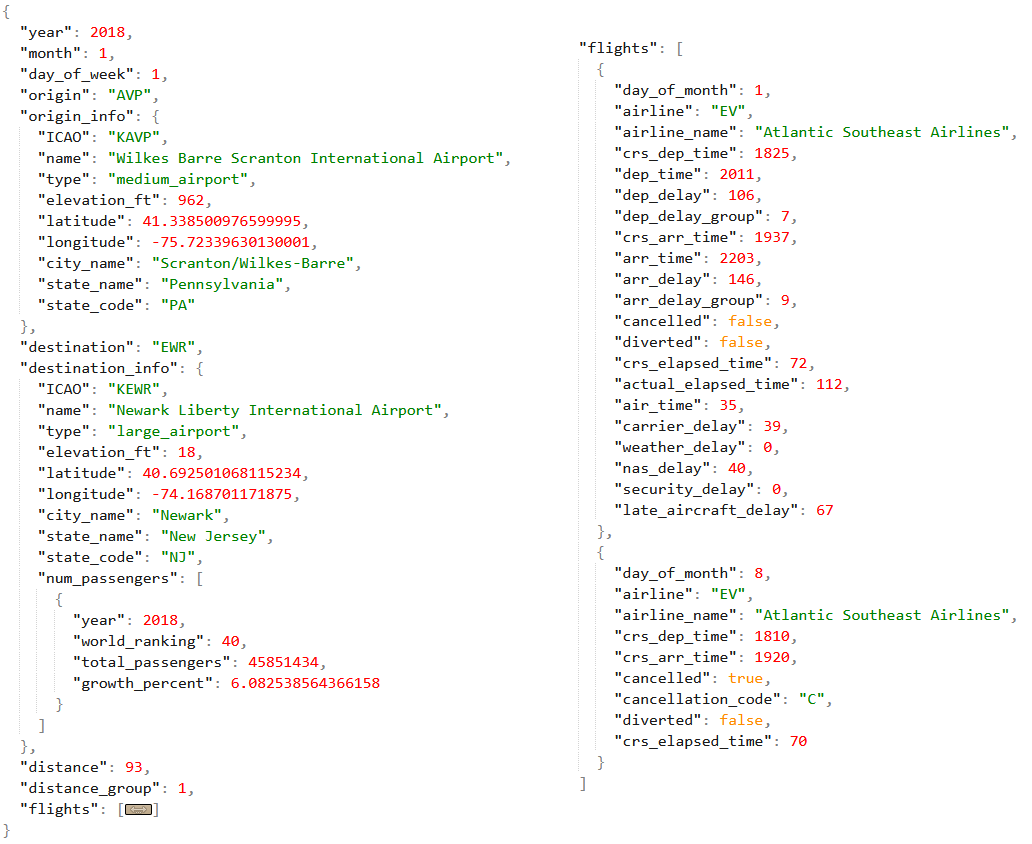
\includegraphics[scale = 0.7]{img/dataMan/JsonSampleDocument.png}\\
  \caption{Esempio di documento json generato dallo script}
\end{figure}
\noindent Da questo esempio è possibile notare come la maggior parte delle informazioni riguardi il volo, inoltre l'arricchimento dati è effettuato tramite embedding di altri documenti, in particolare i campi ``origin\_info'' e ``destination\_info'' contengono tutte le informazioni sugli aeroporti e laddove presente la lista contenente le informazioni sul numero di passeggeri servito negli anni. Il raggruppamento dei dati effettuato inizialmente permette di inserire queste informazioni una sola volta per ogni documento in quanto i voli al suo interno hanno in comune partenza ed arrivo, in questo modo si evitano duplicazioni e si riesce a risparmiare spazio. Mentre l'informazione aggiuntiva sul nome della compagnia aerea è inserita come ulteriore campo in ogni documento relativo al volo.\\
Si può inoltre notare, come già descritto, che il documento non ha una struttura unica e fissa infatti alcuni campi sono inseriti soltanto se assumono un valore valido come evidenzia il caso del secondo volo presente nella lista dove ``mancano'' le informazioni sugli orari effettivi del volo in quanto cancellato.

\section{Gestione del volume}
Per quanto riguarda lo storage dei dati è risultata determinante la necessità di gestire alti volumi di dati e quindi offrire una buona scalabilità. La prima idea, quindi, è stata quella di immagazzinare le informazioni in un database a grafo, come ad esempio Neo4J, in quanto la struttura dei voli si adattava molto bene a questa particolare organizzazione, tuttavia questa tipologia di database non offre una buona scalabilità e quindi non si adattava particolarmente al nostro caso specifico.
Per questa motivazione, abbiamo scelto per lo storage dei dati MongoDB che garantisce una buona scalabilità.\\
Nello specifico, una volta caricati tutti i documenti tramite lo script, si è raggiunto un totale di 4.78GB caricati nel database.

\subsection{L'architettura di MongoDB}
Per gestire l'aspetto del volume si è implementato il metodo del partizionamento dei dati su diverse macchine, questa metodologia, nel caso di MongoDB, prende il nome di \textit{sharding}. L'utilizzo dello sharding abilita la scalabilità orizziontale, che permette al sistema di scalare al crescere dei dati suddividendo il carico applicativo su più macchine. Questo permette di gestire un aumento dei dati o una richiesta di miglioramento delle performance aggiungendo nuove macchine in base alle necessità senza dover continuamente aggiornare l'hardware di un singolo server che richiederebbe aggiornamenti molto costosi. \\
Le componenti principali per lo sharding su Mongo sono le seguenti:
\begin{itemize}
    \item \textbf{Shard}. Ogni shard contiene un sottoinsieme dei dati, nel nostro caso ogni shard è stato implementato come un replica set per garantire anche la tolleranza al partizionamento.
    \item \textbf{Mongos}. Agisce come un router, fornisce l'interfaccia tra le apllicazioni client e lo sharded cluster. 
    \item \textbf{Config server}. Memorizza i metadata e le impostazioni di configurazione per il cluster. Anche il config server è stato implementato come un replica set, in quanto dalla versione 3.4 di Mongo il metodo di mirroring (SCCC) è stato sostituito dal replica set (CSRS) come riportato dalla documentazione ufficiale, permettendo così un miglioramento nei protocolli di scrittura e lettura.
\end{itemize}
Organizzata l'architettura di base e definito il numero di shard si è definita la strategia di sharding, dato che il numero di voli era pressoché costante nei diversi mesi dell'anno si è optato per suddividere i diversi mesi in shard ben specifici in questo modo oltre a garantire il bilanciamento tra i diversi shard si sa con precisione dove verranno effettivamente caricati i dati. La sharded-key è dunque il valore del mese ed è stato suddiviso come:
\begin{itemize}
    \item \textbf{Shard1}. Contiene i mesi tra Gennaio e Aprile
    \item \textbf{Shard2}. Contiene i mesi tra Maggio e Settembre
    \item \textbf{Shard3}. Contiene i mesi tra Ottobre e Dicembre.
\end{itemize}
Con questa suddivisione al termine del caricamento il bilanciamento dei dati nei diversi shard risulta equivalente, tanto è vero che ogni shard contiene circa il 33\% dei dati. Si riporta di seguito l'architettura finale ottenuta:
\begin{figure}[H]
    \begin{center}
      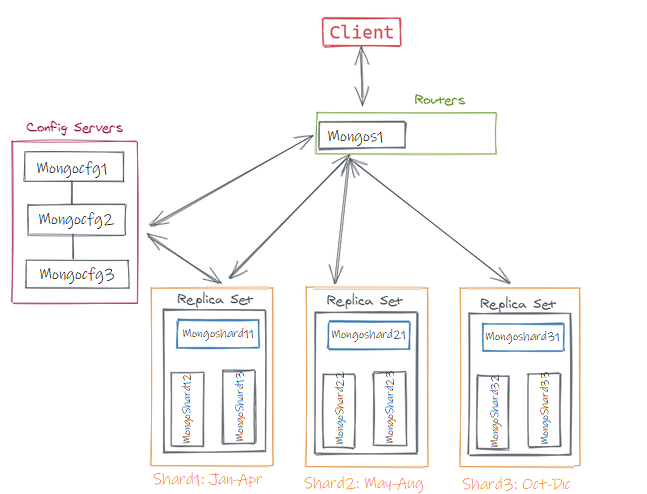
\includegraphics[scale = 0.8]{img/dataMan/sharding-and-replica-sets.png}\\
      \caption{MongoDB architettura sharding}
    \end{center}
\end{figure}

\subsection{Testing dell'architettura}
Per verificare il corretto funzionamento dell'architettura durante la fase di caricamento sono state eseguite, in automatico sfruttano la libreria PyMongo, quattro differenti query che permettessero di controllare il tempo di risposta. Le query eseguite sono:
\begin{itemize}
    \item \textbf{Query1}. Ritorna il ritardo medio di tutti i voli.
    \item \textbf{Query2}. Ritorna il ritardo medio di tutti i voli per una compagnia aerea specifica (EV nel test).\footnote{Questa query è stata aggiunta in un secondo momento e dunque si hanno solo dei risultati parziali come si nota anche dal grafico.}
    \item \textbf{Query3}. Ritorna il ritardo medio di tutti i voli tra gli aereoporti di San Francisco (SFO) e Los Angeles (LAX)
    \item \textbf{Query4}. Ritorna il ritardo medio di tutti i voli nell'anno 2018.
\end{itemize}
Nell'esecuzione di queste query è risultato fondamentale il comando ``\$unwind'' che ha permesso di decomporre l'array contenente le informazioni sui voli in singoli documenti così da poter interrogare anche i campi presenti al suo interno, si riporta di seguito a scopo esemplificativo il codice utilizzato per la terza query:
\vspace{-7pt}
\begin{verbatim}
db.flight.aggregate([{"$match": {"origin": "SFO", "destination": "LAX"}},
                     {"$unwind": "$flights"},  
                     {"$group": {"_id": "_id", 
                                "average": {"$avg": "$flights.arr_delay"}}}, 
                     {"$project": {"_id":0, "average":1}}])
\end{verbatim}
\vspace{-7pt}
Il comando ``\$match'' permette di selezionare in partenza gli aereoporti desiderati, riducendo così la complessità della query. Successivamente l'array flights viene decomposto col comando ``\$unwind'' e ne viene calcolato il tempo medio sul ritardo in arrivo, infine viene proiettato il solo valore medio del ritardo ma è possibile estendere questo comando e ritornare maggiori informazioni se necessario.\\
Il grafico sottostante riporta l'andamento dei tempi di risposta, in secondi, delle query man mano che i dati venivano caricati:
\begin{figure}[H]
\begin{center}
  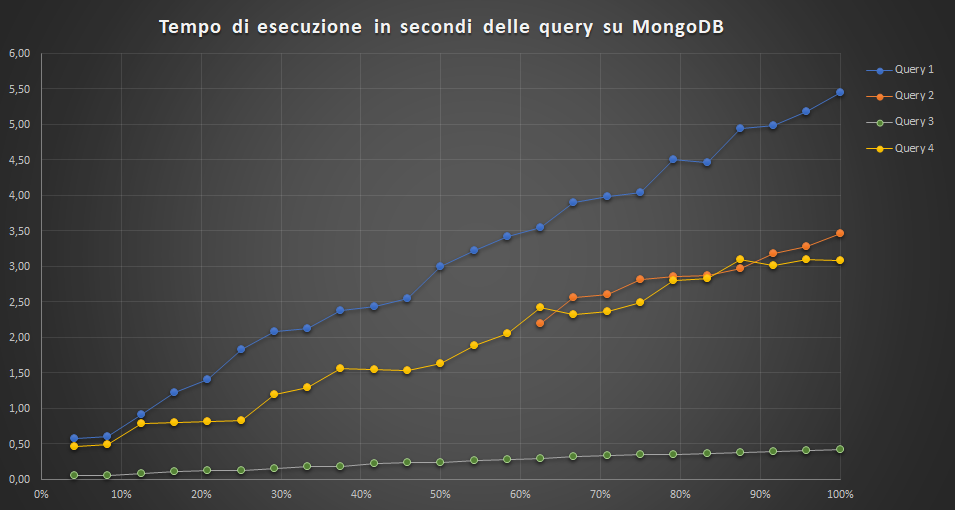
\includegraphics[scale = 0.52]{img/dataMan/QueryTime.png}\\
  \caption{Tempi di risposta di quattro differenti query\protect\footnotemark }
\end{center}
\end{figure}
\footnotetext{La linea tra i diversi punti del grafico non rappresenta valori reali, è solo un aiuto per la comprensione dell'andamento generale.}

\noindent Come si può notare dal grafico nessuna delle query cresce linearmente con l'inserimento dei dati, dunque il partizionamento dei dati risulta efficiente, inoltre si può notare che le query 2,3 e 4 che richiedono una specifica più precisa e realistica risultano particolarmente performanti. In particolare, la query1 registra un maggior incremento nel tempo richiesto per l'esecuzione all'aumentare dei dati, tuttavia rimane distante da un andamento lineare, infatti vi sono alcune fasi in cui i valori rimangono costanti. Inoltre questa query risponde ad una richiesta diversa da quelle prefissateci in partenza, ovvero di cercare un periodo o una compagnia migliore per viaggiare.

\subsection{Conclusioni ed osservazioni}
Come si può notare dai risultati ottenuti nella fase di testi la strategia di sharding adottata risulta efficiente e il database riesce a rispondere bene all'aumento di volume richiesto. Tuttavia estendendo gli anni d'interesse potrebbe essere troppo stringente limitare la suddivisione a soli tre shard organizzati nel modo proposto in quanto ogni singolo anno corrisponde a circa 2.5GB. In tal caso potrebbe essere necessario aggiungere ulteriori shard e modificare il la strategia di sharding suddividendo maggiormente i mesi o includendo anche un range per la settimana o i giorni in questo modo i dati verrebbero maggiormente suddivisi alleggerendo i singoli shard. Questa modifica non comporterebbe un lavoro eccessivo e soprattutto non richiederebbe di riempire nuovamente il database ex-novo in quanto MongoDB mette a disposizione degli appositi comandi come ``sh.updateZoneKeyRange()'' e permette di rivedere e modificare i range di valori precedentemente fissati. Una volta modificati i range, ed eventualmente creati i nuovi shard, la migrazione dei documenti verso lo shard corretto sarà gestita automaticamente anche grazie al bilanciamento automatico dei dati.

\newpage
\part{Data Visualization}
Dopo aver gestito la parte relativa ai dati, abbiamo creato tre diverse dashboard per mostrare i risultati, attraverso l'utilizzo del software Tableau Desktop.

\section{Le infografiche realizzate}
In fase di studio ci si è posti le seguenti domande:
\begin{itemize}
    \item Le compagnie aeree sono tutte uguali?
    \item Esiste un periodo o una destinazione migliore per viaggiare?
    \item L'andamento dei ritardi rimane costante nei diversi anni?
\end{itemize}
L'obiettivo delle nostre infografiche è quello di provare a rispondere a queste domande, per farlo abbiamo realizzato diverse visualizzazioni che permettessero di evidenziare le diverse situazioni.
Si ha iniziato evidenziando il ritardo medio per ogni compagnia aerea, successivamente si è passati a visualizzare l'andamento giornaliero e mensile e i ritardi accumulati nei singoli aeroporti, infine è stato approfondito lo studio mettendo in risalto la percentuale di ritardo tra un anno e l'altro, indicando eventuali voli dirottati o annullati che si sono verificati per ogni mese. Le infografiche realizzate sono state poi inserite a coppie all'interno di apposite dashboard per permettere all'utente di avere un quadro complessivo più chiaro delle varie informazioni.\\
Questa analisi verrà descritta con maggior dettaglio nelle prossime pagine, concludendo con statistiche sui questionari e i test.
Inoltre, si precisa che si è scelto di utilizzare la media come indice di sintesi al fine di non trascurare eventuali valori estremi, e avendo considerato anche che nella letteratura per questo particolare contesto si tende proprio a preferire la media agli altri indici.

\subsection{Ritardo medio per compagnia aerea a livello annuale e mensile}
Sono stati analizzati i ritardi medi riferiti al periodo 2018-2019 associati a ciascuna compagnia aerea, per determinare se vi sia una compagnia migliore per viaggiare sia a livello globale sia per dei mesi specifici. 

\subsubsection{Descrizione delle infografiche}
Per questa analisi sono state realizzate due visualizzazioni che permettono di analizzare in modo più dettagliato la situazione a livello di ogni singola compagnia e a livello complessivo.\\
La prima visualizzazione attraverso uno scatterplot permette di individuare velocemente le peggiori e migliori compagnie a livello di performance grazie al loro posizionamento nel grafico. In aggiunta, è stata riportata la banda di normalità con confidenza al $95\%$ che permette di capire quanto una compagnia si discosti dal rendimento ``comune''.
La seconda visualizzazione invece permette di verificare l'andamento mensile del ritardo in arrivo di ogni singola compagnia aerea.\\
In entrambe le visualizzazioni è stato adottato oltre al posizionamento all'interno del grafico anche il visual cue del colore che denota l'evoluzione del ritardo medio attraverso una scala monocromatica dal rosso chiaro al rosso scuro rendendo visibile le performance di ogni compagnia e il mese ideale per viaggiare. Inoltre, attraverso i controlli posti a lato è possibile selezionare l'anno d'interesse ed eventualmente anche un sottoinsieme di compagnie aeree di proprio interesse per una verifica più mirata. Inoltre, la selezione della singola compagnia aerea è effettuabile pure cliccando su uno specifico pallino a scelta da una qualsiasi delle due visualizzazioni,oltre che utilizzando l'apposito filtro. Una volta selezionata la o le compagnie aeree d'interesse le altre saranno eliminate momentaneamente da entrambe le visualizzazioni offrendo così un confronto più semplice ed intuitivo.

\subsubsection{Commento delle infografiche}
La prima visualizzazione mostra un andamento piuttosto stabile in entrambi gli anni per quanto riguarda le compagnie ``migliori'', infatti nel 2018 le compagnie Hawaiian Airlines ed Alaska Airlines sono riuscite a distinguersi per le ottime performance arrivando addirittura in  anticipo rispetto a quanto programmato. Nel 2019 la situazione rimane pressoché invariata con però la compagnia Alaska Airlines che registra oltre cinque minuti di ritardo in partenza. Per quanto riguarda le quattro principali compagnie USA (Delta Airlines, American Airlines, United Airlines e Southwest Airlines),la Delta Airlines risulta la migliore anche se in partenza è caratterizzata da un ritardo medio pressoché equivalente alle altre, data la vicinanza alla banda di normalità. 
Dall'altro lato, la compagnia che ha accumulato nel corso del 2018 il più alto ritardo è la Frontier Airlines con ritardi alti soprattutto nel mese di giugno. Nel 2019 è invece l'Atlantic Southeast Airlines a detenere il primato di peggior compagnia aerea, mentre la Frontier registra un netto miglioramento delle proprie performance. In questo stesso anno si registra anche un peggioramento della JetBlue Airlines soprattutto nei ritardi in partenza.\\
Questa tipologia di grafico mette anche in risalto il fatto che non sempre un alto ritardo in partenza corrisponde ad un arrivo ritardato, questo perché spesso qualche minuto di ritardo è riassorbito durante il volo soprattutto nelle tratte a lunga percorrenza.\\
La seconda visualizzazione invece permette di verificare l'andamento mese per mese delle compagnie che in generale evidenzia che nei mesi tra giugno e agosto si verificano i ritardi più consistenti dovuti al traffico aereo più intenso (i vacanzieri aumentano), così come  possibili scioperi del personale, temporali estivi, guasti e manutenzioni ai velivoli. Un discorso analogo pare valere anche per i mesi di dicembre e gennaio caratterizzati da molti giorni di festa.

\begin{figure}[H]
    \hspace{-33pt}
    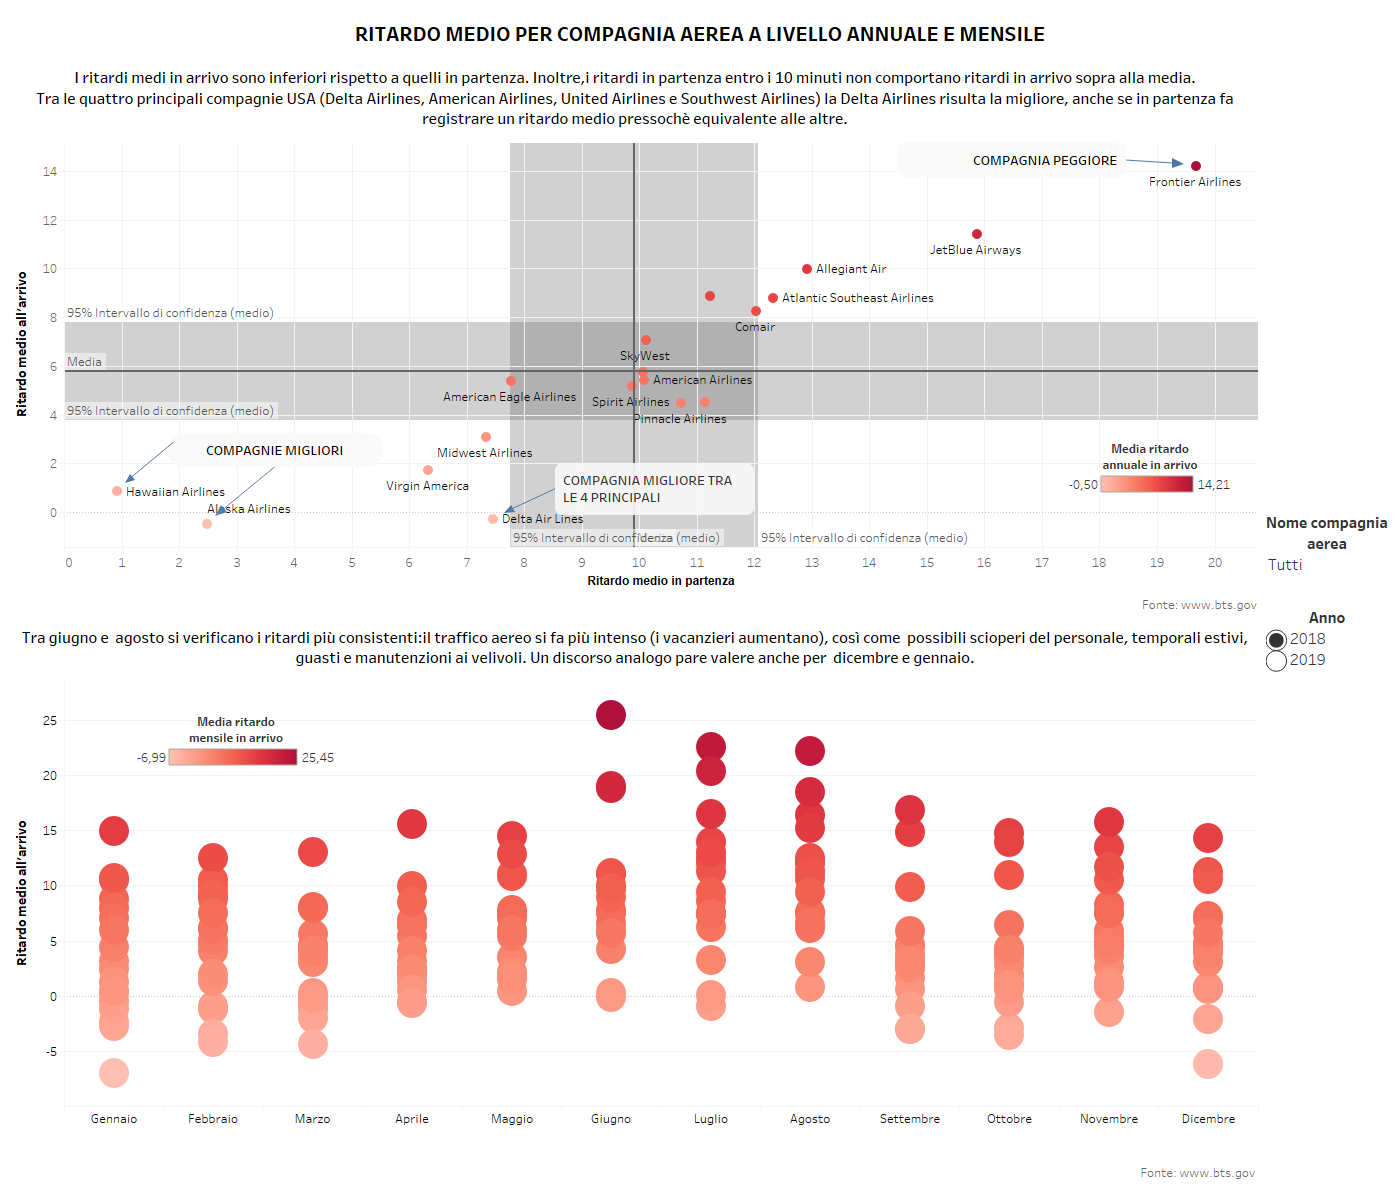
\includegraphics[scale = 0.53]{img/dashboard/Dashboard1.png}
    \caption{Infografiche prima dashboard}
\end{figure}

\newpage
\subsection {Analisi dei ritardi a livello geografico e temporale}
Abbiamo effettuato un'analisi approfondita del ritardo medio per ciascun anno per fare un confronto e delineare se vi sia un aeroporto o uno stato particolarmente migliore o peggiore di altri e se esistano dei periodi ideali sia a livello mensile che settimanale per viaggiare.

\subsubsection{Descrizione delle infografiche}
La prima visualizzazione presente in questa dashboard visualizza l'andamento a livello territoriale dei singoli aeroporti permettendo così all'utente di verificare le performance degli aeroporti o di stati di proprio interesse. Il ritardo medio di ogni aeroporto, se non vi sono particolari filtri impostati, è calcolato su tutti i giorni e tutti i mesi dell'anno scelto. In questo caso sono stati adottati due visual cues: i cerchi rappresentanti i singoli aeroporti infatti l'aerea aumenta con l'aumentare del ritardo medio in arrivo, inoltre si ha optato anche per usare una scala di colori dall'azzurro chiaro al rosso scuro per denotare l'andamento del ritardo medio in arrivo, in questo caso l'azzurro è stato adottato per rappresentare gli arrivi anticipati nel tempo.
La seconda visualizzazione invece renderizza in una matrice l'andamento dei ritardi a livello complessivo per tutti gli aeroporti statunitensi. Nello specfico, le righe della matrice riportano i giorni della settimana mentre le colonne i mesi dell'anno. Utilizzando una scala si colori si ha ottenuto una visualizzazione che permette agli utenti di verificare a livello visivo quale sia la giornata o il mese con minor ritardo in media, a tal fine vengono anche riportati testualmente il valore minimo e massimo registrati (che si adatta e aggiorna in base ai periodi selezionati). Anche in questo caso, è stata adottata una scala di colori dall'azzurro al rosso per denotare l'aumento del ritardo medio in arrivo.\\
Nella parte destra della dashboard sono a disposizione degli appositi filtri che permettono di semplificare la visualizzazione proposta andando a visualizzare informazioni più dettagliate di proprio interesse. \'E infatti possibile selezionare i mesi e/o i giorni a piacere, ma anche degli stati specifici. Comunque, una volta effettuata la selezione le due visualizzazioni si riadattano in automatico per visualizzare quanto richiesto dall'utente. Anche in questo caso, come per la prima dashboard, è possibile effettuare la selezione di giorno e mese direttamente cliccando sui blocchi d'interesse della matrice. Infine, ovviamente è anche possibile selezionare l'anno per l'analisi.

\subsubsection{Commento delle infografiche}
A livello territoriale si evidenzia, per entrambi gli anni, che le aree più densamente abitate (ovvero le coste e la parte orientale) tendono a mostrare un'elevata concentrazione di ritardi.
Mentre dal secondo grafico si evince che i mesi di marzo e settembre,in entrambi gli anni, sembrano i mesi migliori per viaggiare, così come il giovedì sembra il giorno migliore. Mentre i mesi estivi (giugno, luglio e agosto) e il lunedì sono caratterizzati da numerosi e intensi ritardi. Si può notare, infatti, un peggioramento tendenzialmente già a partire dal mese di maggio, mentre settembre e registra un netto miglioramento in termini di ritardo. A livello complessivo, dunque, si può concludere che i primi 5 mesi dell'anno siano caratterizzati da ritardi un po' meno consistenti rispetto agli ultimi 5 mesi.\\
Utilizzando il filtro annuale è anche possibile effettuare un confronto tra i due anni che mostra come il 2019 sia caratterizzato da un peggioramento rispetto all'anno precedente. Questa analisi sarà però affrontata in modo più chiaro e diretto nelle visualizzazioni successive.

\begin{figure}[H]
    \hspace{-33pt}
    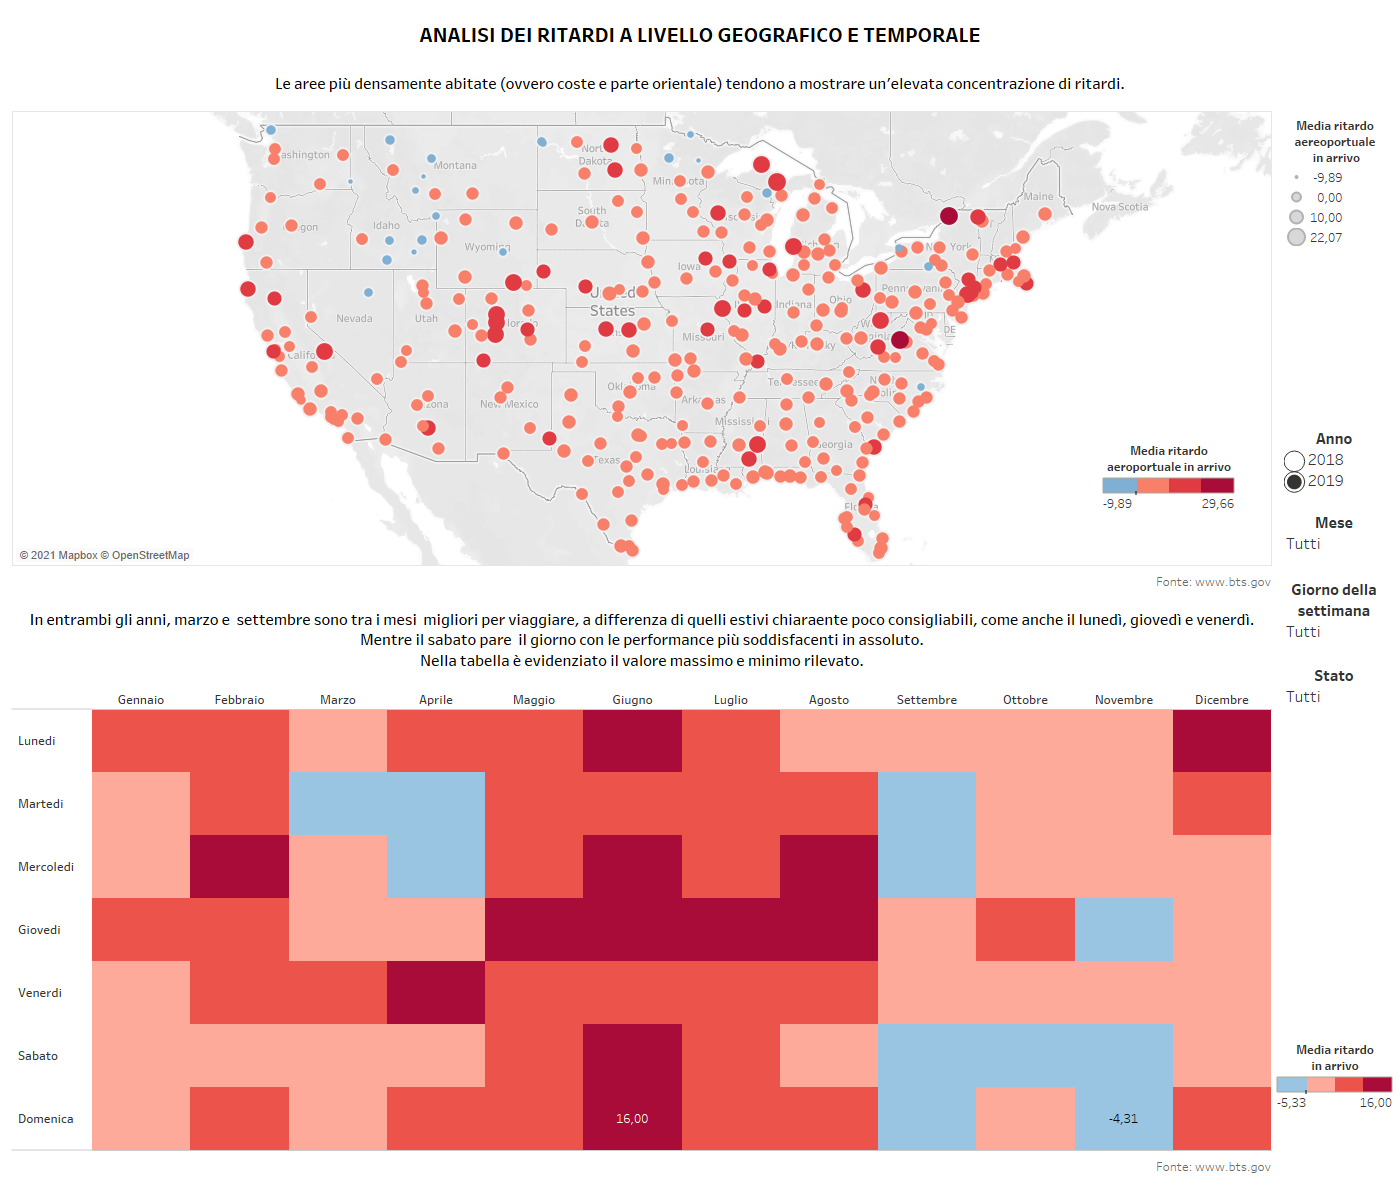
\includegraphics[scale = 0.53]{img/dashboard/Dashboard2.png}
    \caption{Infografiche seconda dashboard}
    \label{dash2}
\end{figure}

\newpage
\subsection {Analisi performance 2019}
Nell'ultima dashboard si è voluta approfondire l'analisi sulle performance dell'anno 2019 per mettere in luce eventuali differenze tra i diversi mesi dell'anno. Inoltre, come anticipato nel commento della dashboard precedente, si è studiata la differenza tra il 2018 e 2019 al fine di verificare se vi sia stato un miglioramento e nel caso in quali periodi dell'anno.

\subsubsection{Descrizione delle infografiche}
Il primo grafico riporta attraverso delle stacked-bar le informazioni sui voli visualizzando a livello percentuale il numero di voli cancellati, dirottati, in ritardo e in orario.
Il secondo grafico invece analizza il cambiamento del ritardo da un anno all'altro, evidenziando con delle barre la percentuale di cambiamento nei vari mesi. In questo caso è stata adottata una scala bicolore dove l'azzurro indica un miglioramento rispetto all'anno precedente, ovvero più voli sono arrivati in orario, mentre il peggioramento è indicato dal colore rosso e dalla barra negativa.\\
In questa dashboard, a differenza delle precedenti, è presente un solo filtro che permette di selezionare un mese specifico, evidenziando a livello percentuale i diversi valori nelle barre dei due grafici. Questa selezione, come sempre, è anche effettuabile cliccando sulle barre nei diversi grafici. Inoltre per il primo grafico data la presenza di percentuali molto piccole e quasi impercettibili alla vista è possibile cliccare anche sulla tipologia di volo d'interesse direttamente dalla legenda colori in alto a destra, che permetterà di osservare chiaramente le percentuali della sezione scelta.

\subsubsection{Commento delle infografiche}
La prima visualizzazione rende evidente che la prevalenza dei voli risulta arrivare in orario anche se una buona percentuale di voli registra comunque ritardi consistenti.\'E inoltre evidente che soltanto una percentuale esigua di voli vengano dirottati, la sezione colorata in arancio scuro che riporta questa percentuale è infatti molto sottile nelle barre e non supera mai lo $0.35\%$ nel 2019, con un lieve picco però tra giugno e luglio (probabilmente per l'aumento del traffico aereo). Infine si può notare come nei mesi di gennaio e di marzo vi sia una più alta percentuale di voli cancellati, rispettivamente il $2.94\%$ e il $2.4\%$. La motivazione, come riportato nel grafico sottostante è dovuta probabilmente alle condizioni meteorologiche avverse di quel periodo.\\
Il secondo grafico, invece, evidenzia come il 2019 nel complesso registri performance molto più negative dell'anno precedente segnando in media un $-15.8\%$ di voli che arrivano in orario. La motivazione di questo peggioramento, come già ipotizzato in precedenza, è appunto probabilmente dovuta ad eventi climatici estremi. Infatti, grazie ad alcune fonti esterne, è stato possibile risalire a quanto accaduto in quel lasso temporale: da fine gennaio a metà marzo in larga parte degli USA si è registrata un'ondata di freddo polare particolarmente intensa che avrebbe quindi causato ritardi più elevati, come evidenziano le barre rosse con percentuali molto elevate; addirittura nel mese di febbraio il numero di voli in ritardo è aumentato di oltre il doppio rispetto al 2018 registrando un $-137\%$. Questo grafico per di più, contrariamente a quanto ci si possa aspettare, evidenzia che nei mesi estivi la percentuale di arrivi in orario è migliorata, registrando un picco nei mesi di settembre e novembre. Come in precedenza una possibile motivazione è da ricercarsi a livello ambientale: solitamente questi mesi sono caratterizzati da grossi incendi che talvolta compromettono a tal punto la visibilità da posticipare i voli. Comunque nel 2019 i cosiddetti "wildfire" si sono verificati in un numero nettamente inferiore rispetto all'anno precedente. 

\begin{figure}[H]
    \hspace{-33pt}
    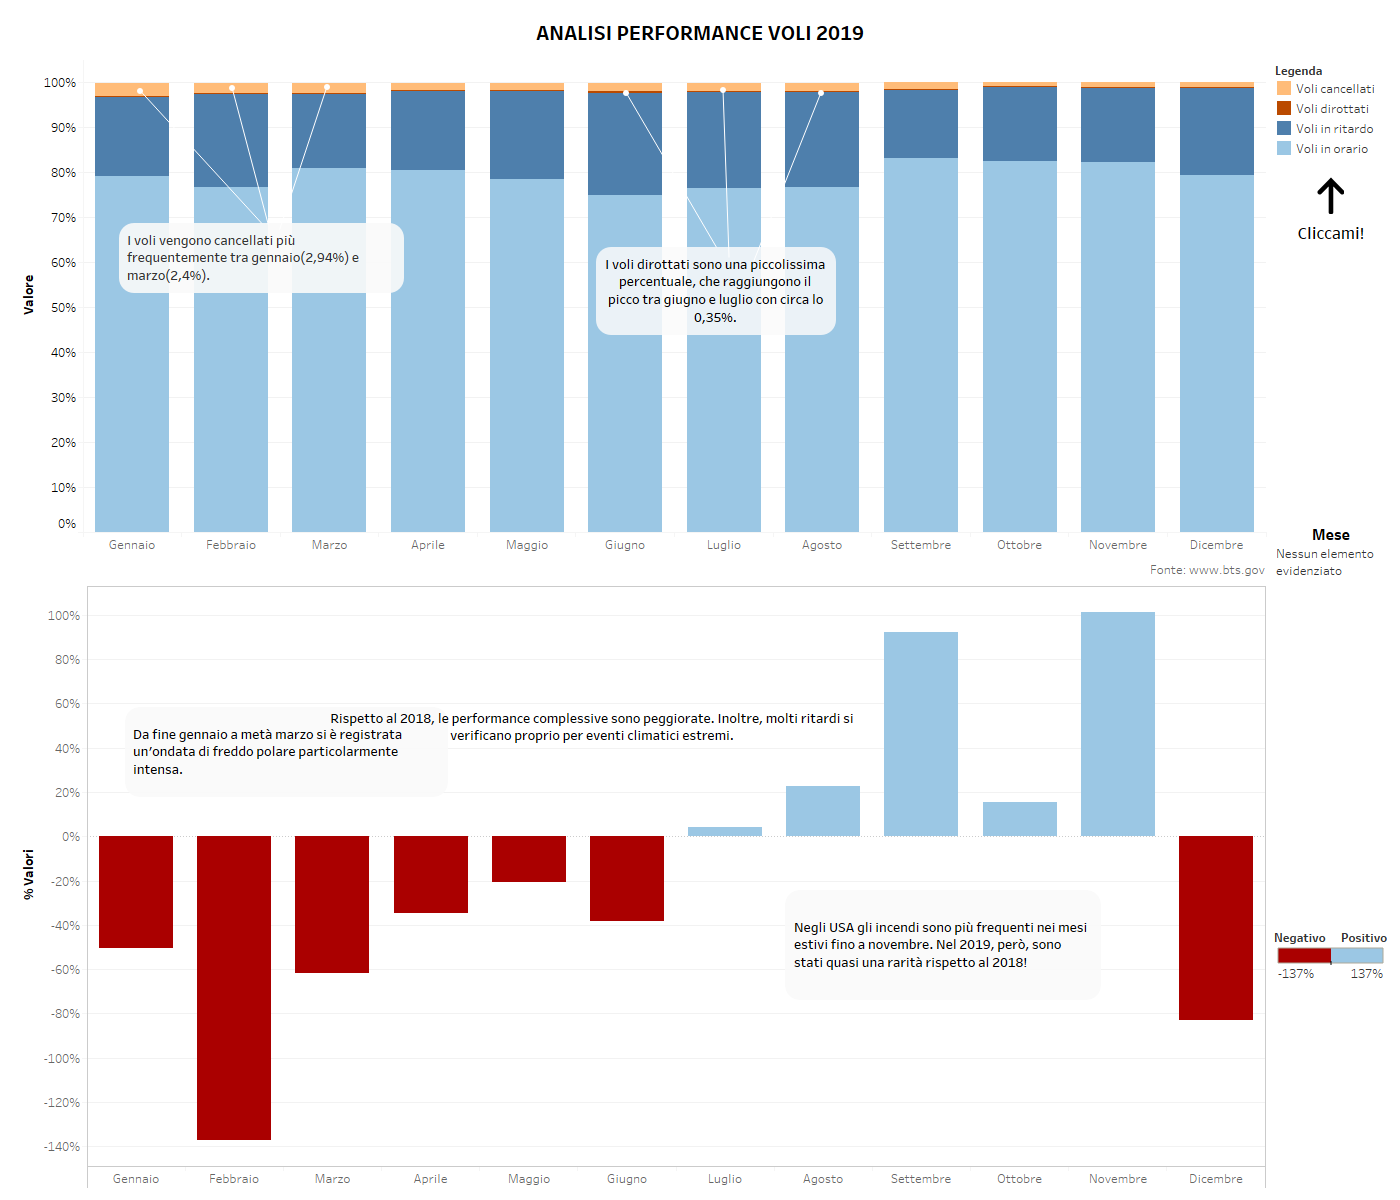
\includegraphics[scale = 0.53]{img/dashboard/Dashboard3.png}
    \caption{Infografiche terza dashboard}
\end{figure}

\subsection{Storia}
Completate le tre dashboard appena descritte si è deciso di realizzare una storia che provasse a guidare l'utente nella visualizzazione e comprensione, ogni dashboard è infatti anticipata da un testo introduttivo che ne spiega lo scopo complessivo e cosa è visualizzato nei singoli grafici.

\newpage
\section{Valutazione euristica delle infografiche}
Una prima analisi delle visualizzazioni è stata continuamente fatta durante il processo di realizzazione delle stesse, infatti essendo il nostro gruppo composto da tre persone con background universitari ed idee differenti ogni decisione finale è arrivata soltanto dopo un dibattito costruttivo all'interno del gruppo. Dopo aver trovato una soluzione interna abbiamo verificato il lavoro condividendolo con un ristretto gruppo di cinque persone per avere un primo riscontro e cercare di migliorare dove possibile le visualizzazioni. Di seguito sono riportati i consigli e le critiche dateci in questa prima fase di valutazione.

\subsection{Prima dashboard}
Per quanto riguarda la prima dashboard, quella sui ritardi medi delle compagnie aeree, ci sono state mosse principalmente due critiche. Inizialmente ci è stato consigliato di posizionare i valori degli assi in ordine decrescente in modo da avere nella parte in alto a destra del grafico le compagnie migliori. La seconda critica, mossa da un paio di utenti, riguarda la pienezza del grafico che, per per gli utenti richiede un maggior lasso di tempo per comprenderlo a pieno.\\
Unendo le critiche ricevute abbiamo deciso di mantenere la convenzione sull'origine e dunque di non modificare gli assi, tuttavia per cercare di facilitare e velocizzare la comprensione abbiamo inserito più context cercando di guidare così gli utenti nella lettura del grafo.

\subsection{Seconda dashboard}
Per quanto riguarda questa dashboard ci sono arrivati diversi consigli. La prima critica riguarda la scelta dei colori, infatti gli utenti avrebbero preferito la coppia Rosso-Verde per identificare peggioramenti e miglioramenti nelle performance, purtroppo quest'accoppiata di colori non è stato possibile utilizzarla per permettere anche ai daltonici di consultare la visualizzazione senza problemi. Questa stessa critica ci è stata mossa anche per la terza dashboard, anche se in maniera meno marcata.\\
L'altra critica riguarda la matrice colori che, secondo alcuni utenti, è risultata troppo ``piena'' e soprattutto senza margini tra le varie celle come mostrato nella \ref{dash2}, abbiamo quindi provato ad inserire dei margini tra celle ottenendo il seguente risultato:
\begin{figure}[H]
    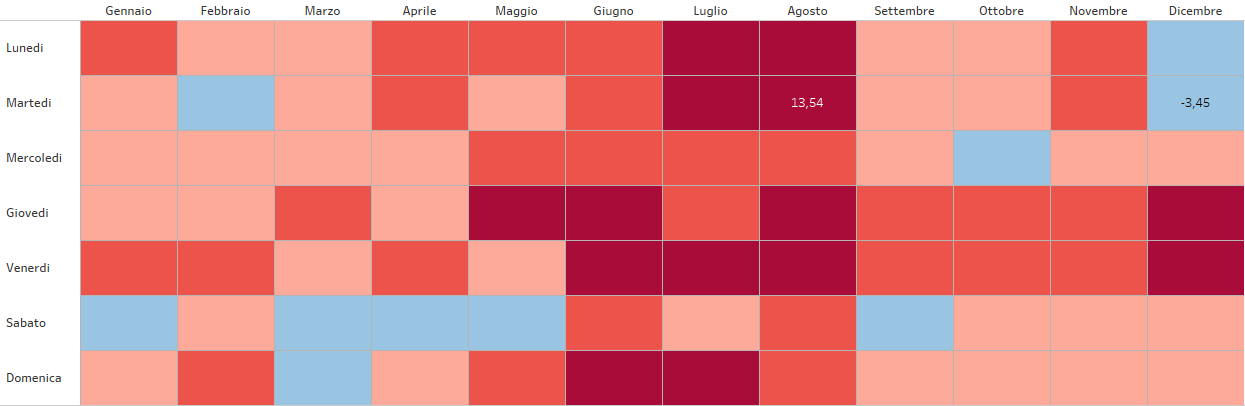
\includegraphics[scale = 0.5]{img/dashboard/tabella_colori_bordo.png}
    \caption{Tabella colori dashboard2 revisionata}
\end{figure}
\noindent Sempre a riguardo della matrice ci è stato detto che probabilmente questa visualizzazione richiede una conoscenza di base sulla statistica per capire come viene colorata la matrice e che magari per le persone meno pratiche sarebbe risultata complessa. Purtroppo per questa critica non abbiamo potuto raccogliere informazioni valide dagli utenti in quanto i pochi, che ci attendiamo non conoscano molta statistica, che siamo riusciti a raggiungere anche attraverso il questionario non hanno evidenziato particolari difficoltà nella comprensione, tuttavia sarebbe interessante ricevere dei feedback più accurati per verificare se sussista o meno questa problematica.\\ 
L'ultima critica invece ha riguardato le scale colori, che riportavano lo stesso nome anche se si riferivano a dati leggermente diversi in quanto nella mappa il ritardo è riferito al singolo aeroporto mentre la matrice riporta un valore complessivo, e i filtri che in alcuni casi non riportavano i valori in ordine alfabetico. La problematica dei filtri è stata corretta, mentre per quanto riguarda le scale colori abbiamo cambiato leggermente il posizionamento per metterle più vicino al grafico d'appartenenza e anche cambiato la descrizione per diversificarle.


\subsection{Terza dashboard}
Questa dashboard non ha ricevuto particolari critiche da parte degli utenti, anche se per alcuni essendo la più facile da comprendere sarebbe meglio scambiarla con la prima e invertire quindi l'ordine delle dashboard. Seguendo questo consiglio abbiamo deciso di inserire la domanda alla fine del questionario psicometrico per la valutazione delle infografiche per capire il pensiero di un numero maggiore di persone, verrà quindi discussa nei capitoli successivi la decisione presa.

\newpage
\section{Questionario psicometrico}
Per quanto riguarda la valutazione dei grafici ci si è serviti anche di un questionario psicometrico per avere un feedback più strutturato e più facilmente analizzabile a livello quantitativo. Si è chiesto, dunque, ad un gruppo di 28 individui di rispondere ad alcune semplici domande. Inizialmente per ogni dashboard, discostandosi leggermente dalla classica scala Cabitza-Locoro, si è domandato una valutazione in termini di utilità, chiarezza, informatività, intuitività e utilità con un punteggio minimo di 1 (pochissimo) e un massimo di 6 (moltissimo). In seguito, sempre con la stessa scala di risposta, si è richiesta anche una valutazione globale della qualità della dashboard.
Successivamente, i risultati sono stati analizzati tramite il software R impiegando sia degli stacked bar chart, con i relativi intervalli di confidenza, che dei correlogrammi.

\subsection{Analisi dei risultati della prima infografica}
La distribuzione dei punteggi pare essere piuttosto omogenea tra le variabili, registrando comunque un picco di voti positivi per l'informatività,al contrario di quanto accade per la  bellezza e l'intuitività. Comunque, per tutte le variabili si può affermare che la proporzione di giudizi negativi sia significativamente inferiore alla metà dei voti.
A livello di correlazione, invece, dal grafico si può notare come la bellezza incida un po' di più rispetto alle altre caratteristiche sulla valutazione complessiva, seguita dall'utilità e dall'intuitività, anche se complessivamente i valori in generale sono abbastanza simili. Inoltre, la correlazione maggiore si è verificata tra bellezza e intuitività, e sempre tra quest'ultima e utilità, anche se in misura leggermente inferiore. Complessivamente, comunque, l'$R^2$ che è stato calcolato relativamente a questa dashboard risulta essere pari a 0.58.
\begin{figure}[H]
    \centering
    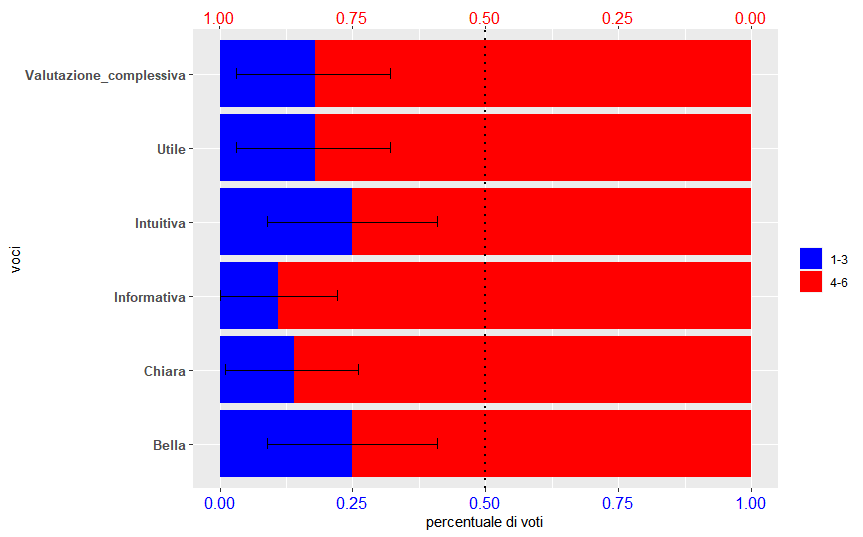
\includegraphics[scale = 0.6]{img/Questionari/StackedBarplot_1.png}
    \caption{Stacked bar chart Dashboard 1}
\end{figure}


\begin{figure}[H]
    \hspace{20pt}
    \vspace{-20pt}
    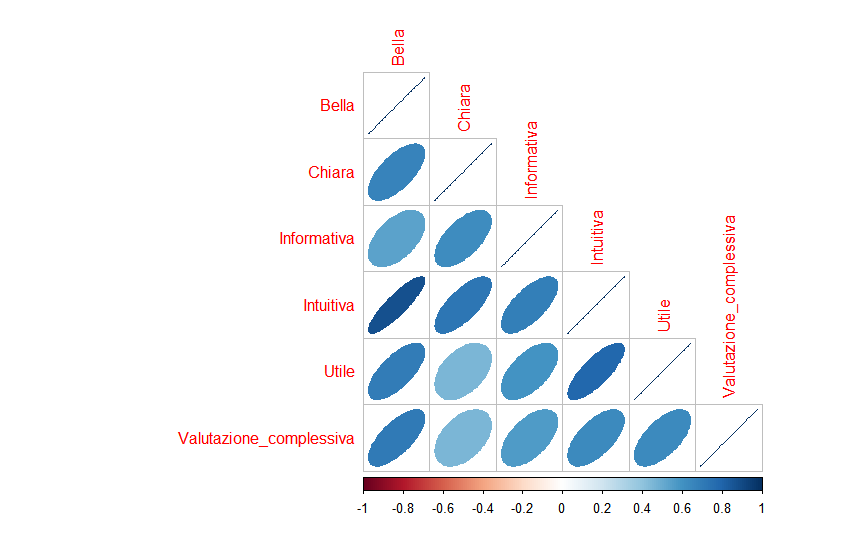
\includegraphics[scale = 0.6]{img/Questionari/Correlogramma_1.png}
    \caption{Correlogramma Dashboard 1}
\end{figure}

\subsection{Analisi dei risultati della seconda infografica}
Innanzitutto,per tutte le variabili si può sottolineare che le proporzioni
dei voti negativi sono significativamente inferiori alla metà dei voti, anche se in modo meno evidente per la bellezza e l'intuitività. Inoltre, stando ai punteggi rilevati i grafici sono stati giudicati decisamente informativi e anche chiari.
Dal correlogramma, in aggiunta, si evince che la bellezza, seguita dall'intuitività, siano le variabili che incidono maggiormente sulla valutazione complessiva, mentre l'informatività meno rispetto alle altre. In questo caso, invece, l' $R^2$ è decisamente più elevato ed è pari a 0.85.
\begin{figure}[H]
    \centering
    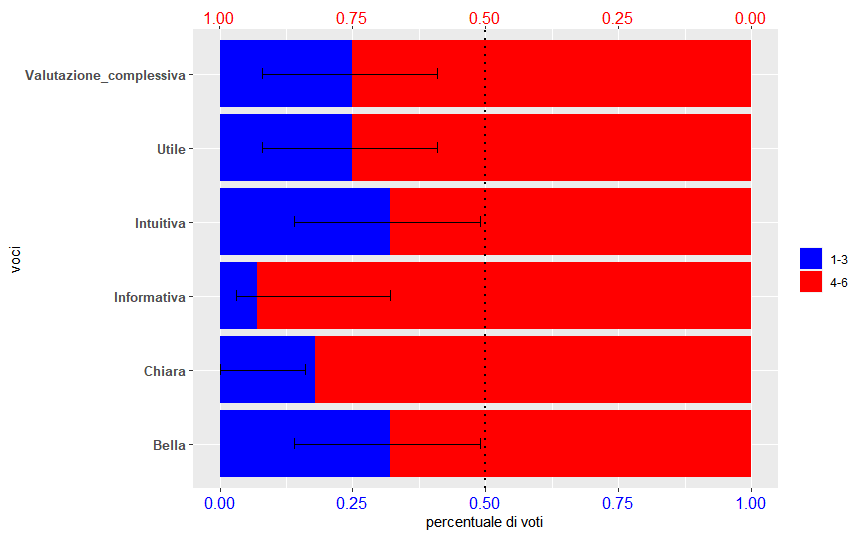
\includegraphics[scale = 0.55]{img/Questionari/StackedBarplot_2.png}
    \caption{Stacked bar chart Dashboard 2}
\end{figure}


\begin{figure}[H]
    \hspace{20pt}
    \vspace{-20pt}
    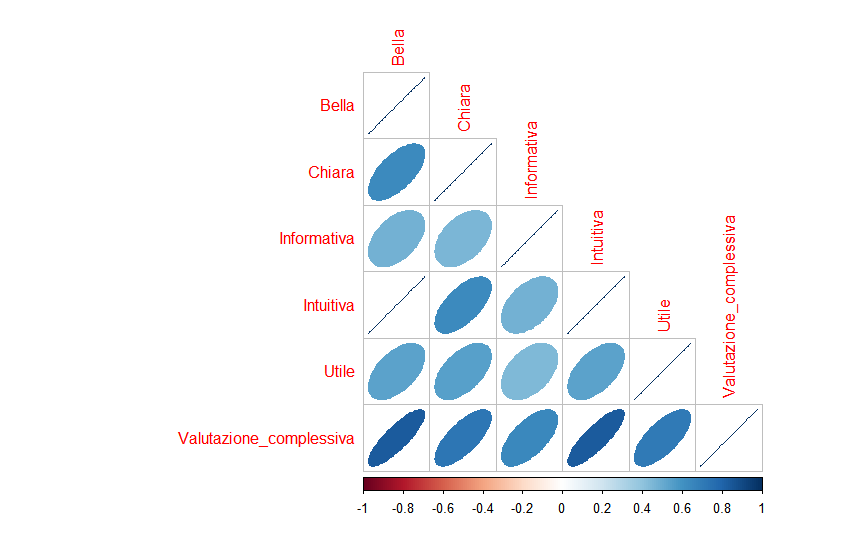
\includegraphics[scale = 0.6]{img/Questionari/Correlogramma_2.png}
    \caption{Correlogramma Dashboard 2}
\end{figure}



\subsection{Analisi dei risultati della terza infografica}
Dal grafico si può vedere chiaramente che tutte le variabili hanno ricevuto una proporzione di voti negativi significativamente inferiore alla metà, tranne nel caso della bellezza. Comunque, si potrebbe affermare che gli utenti hanno ritenuto questa dashboard particolarmente informativa.
Per quanto riguarda il correlogramma, infine, si può notare che ad influenzare di più la valutazione complessiva sono ancora la bellezza e l'informatività, mentre l' $R^2$ riferito a quest'ultima dashboard è pari a 0.86.

\begin{figure}[H]
    \centering
    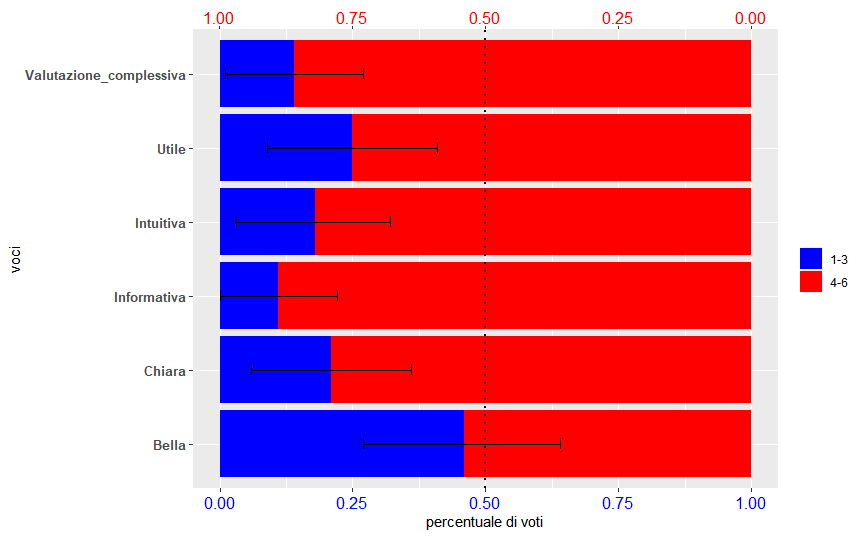
\includegraphics[scale = 0.55]{img/Questionari/StackedBarplot_3.png}
    \caption{Stacked bar chart Dashboard 3}
\end{figure}


\begin{figure}[H]
    \hspace{20pt}
    \vspace{-20pt}
    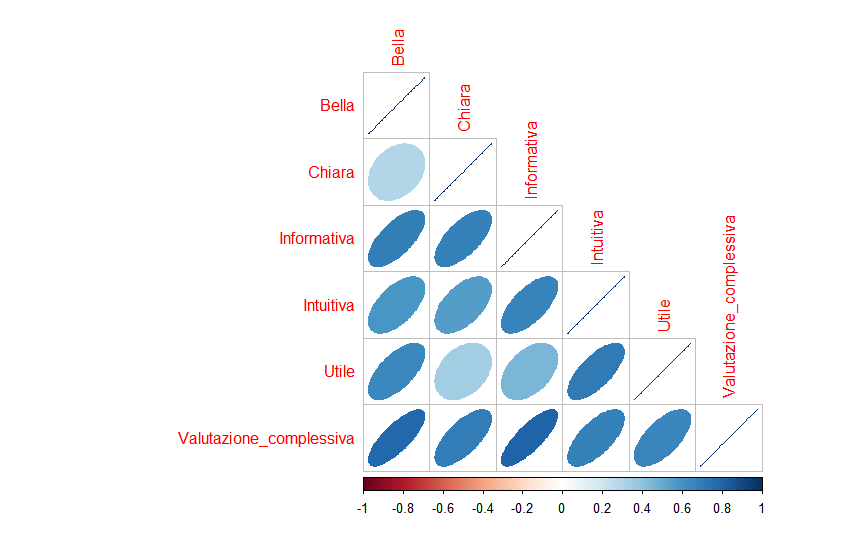
\includegraphics[scale = 0.6]{img/Questionari/Correlogramma_3.png}
    \caption{Correlogramma Dashboard 3}
\end{figure}

\newpage
\section{Test utenti}
Con lo scopo di valutare al meglio le infografiche realizzate abbiamo sottoposto ad un secondo campione composto da 12 utenti alcune domande più specifiche che richiedessero di interagire con i grafici. Le domande sono state suddivise per dashboard e oltre a valutare la correttezza della risposta dataci dai singoli utenti è stato valutato anche il tempo impiegato, ogni volta che l'utente visualizzava una nuova domanda in automatico partiva il cronometro corrispondente. Per avere un confronto rispetto ai tempi degli utenti abbiamo compilato noi stessi per primi questo secondo questionario in modo da ottenere una tempistica di riferimento. I risultati sono stati analizzati tramite il software R realizzando degli stacked bar chart con la percentuale di errore e dei violin plot per ogni domanda, riportando sia il tempo impiegato per rispondere sia la correttezza o meno della risposta. Nei violin plot che seguono la linea continua è il riferimento rispetto al tempo medio impiegato da noi per rispondere alla domanda mentre le due linee tratteggiate delimitano la banda di normalità, allo stesso modo negli stacked bar chart è riportata la banda di normalità e la percentuale al 5\%.

\subsection{Task prima dashboard}
Il task proposto per la prima dashboard è il seguente:
\begin{itemize}
    \item Quale ritieni che sia il mese migliore per la compagnia Delta Airlines nell'anno 2019?
\end{itemize}
La domanda richiedeva dunque di filtrare correttamente sia l'anno sia la compagnia aerea per visualizzare nella sezione inferiore i dati corretti. Si riporta di seguito il risultato ottenuto dagli utenti:
\begin{figure}[H]
    \centering
    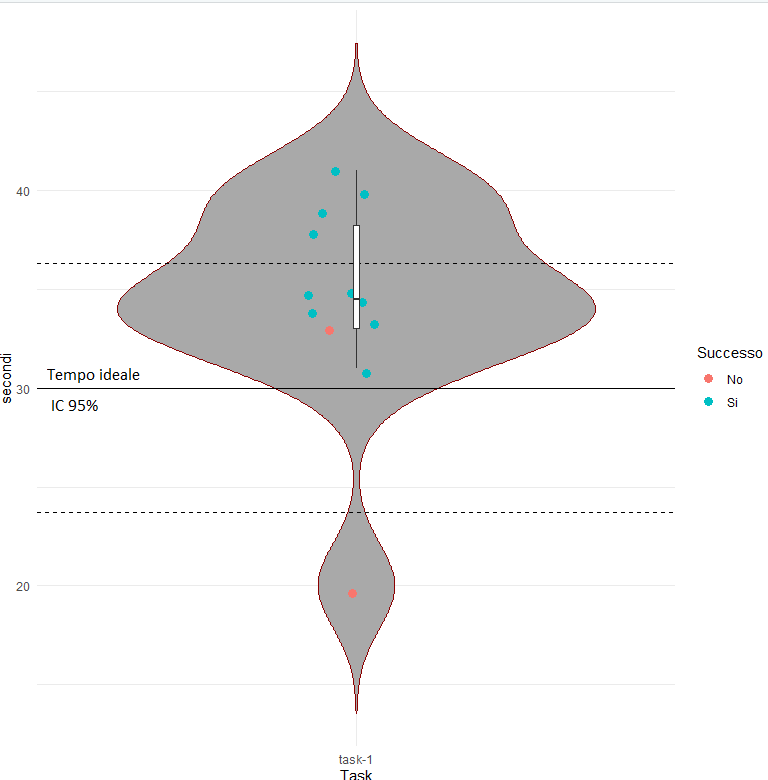
\includegraphics[scale = 0.5]{img/task/Dash1_task.png}
    \caption{Task prima dashboard}
\end{figure}
\noindent Gran parte degli utenti impiega circa 34 secondi per rispondere, e si sono registrati due errori nelle risposte di cui uno probabilmente dettato dalla fretta in quanto il tempo di risposta è molto al di sotto del tempo medio previsto.\\
Inoltre, ci è stato segnalato dagli utenti che in alcuni casi il filtraggio non risultava immediato per via della connessione internet e dunque l'utente era costretto ad aspettare prima di poter rispondere, aumentando così il tempo necessario.\\
Si riporta di seguito lo stacked bar chart con la percentuale di risposte corrette ricevute:
\begin{figure}[H]
    \centering
    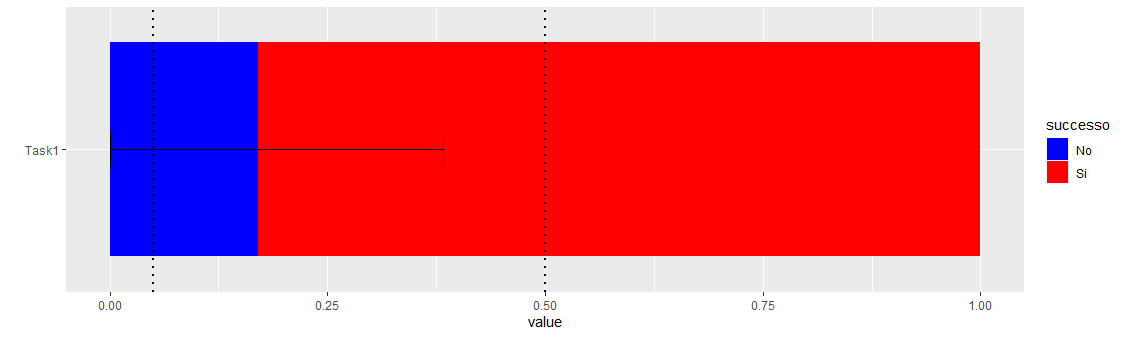
\includegraphics[scale = 0.45]{img/task/Dash1_task_ErrorBar.png}
    \caption{Stacked bar chart task1}
\end{figure}


\subsection{Task seconda dashboard}
Per questa dashboard sono stati proposti due task:
\begin{itemize}
    \item Quale ritieni che sia, per il mese di Marzo 2019, il giorno migliore per viaggiare?
    \item Secondo te, escludendo lo stato della California, in quale giorno è stato registrato il minor ritardo nell'anno 2019?
\end{itemize}
Il due task si differenziano per complessità, il primo infatti non richiedeva alcun filtraggio ma soltanto di analizzare correttamente la matrice colori presente nella sezione inferiore, il secondo task invece chiedeva un impegno ed una comprensione maggiore della richiesta da parte degli utenti. Questa differenza si nota abbastanza evidentemente anche nei violin plot:  
\begin{figure}[H]
	\begin{minipage}[b]{0.48\textwidth}
		\centering
		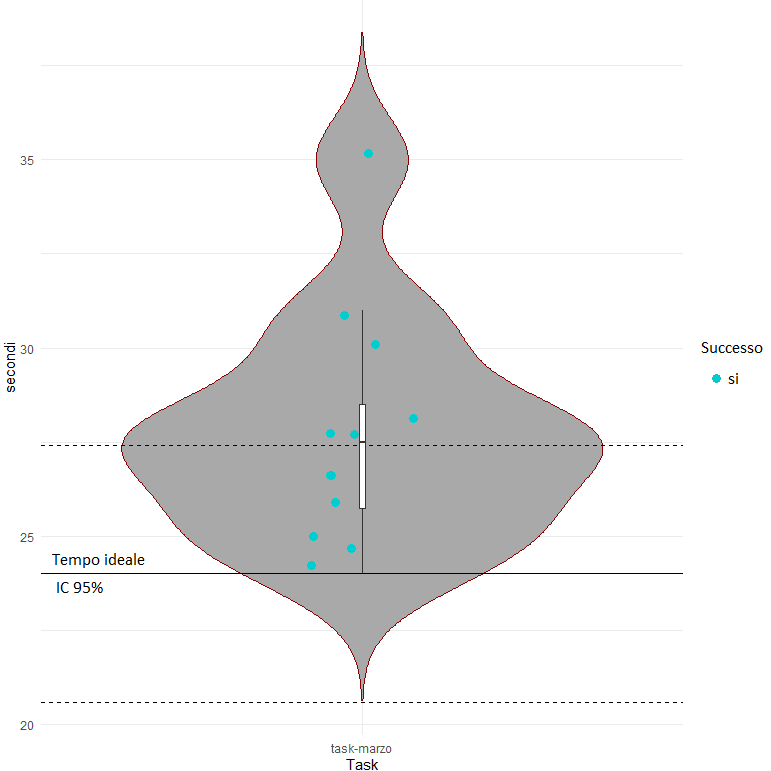
\includegraphics[width=\textwidth, height=7cm]{img/task/Dash2_TaskMarzo.png}
        \caption{Task1 seconda dashboard}
	\end{minipage}
	\hfill
	\begin{minipage}[b]{0.48\textwidth}
		\centering
		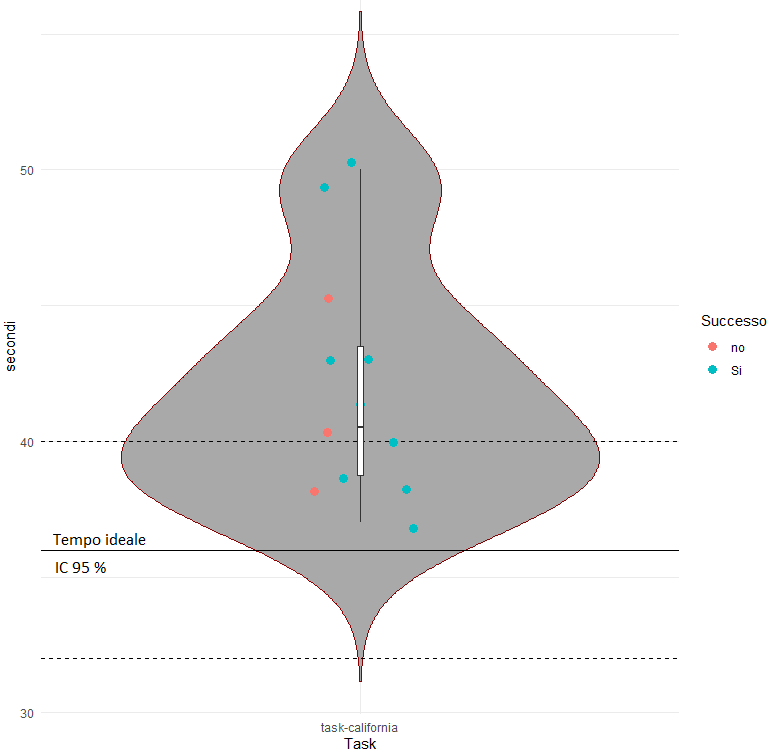
\includegraphics[width=\textwidth, height=7cm]{img/task/Dash2_TaskCalifornia.png}
        \caption{Task2 seconda dashboard}
	\end{minipage}
\end{figure}
\noindent Per il primo task, riportato nella figura di sinistra, non sono stati registrati errori e il tempo medio di risposta si attesta intorno ai 27 secondi con diversi utenti che rientrano nella banda di normalità rispetto al nostro tempo medio di risposta.\\
Il secondo task, più complesso, ha fatto registrare un tempo di risposta medio più elevato, intorno a 41 secondi, e 3 errori da parte degli utenti.\\
Si riporta di seguito lo stacked bar chart con la percentuale di risposte corrette ricevute per il secondo task in quanto nel primo non sono presenti risposte errate:
\begin{figure}[H]
    \centering
    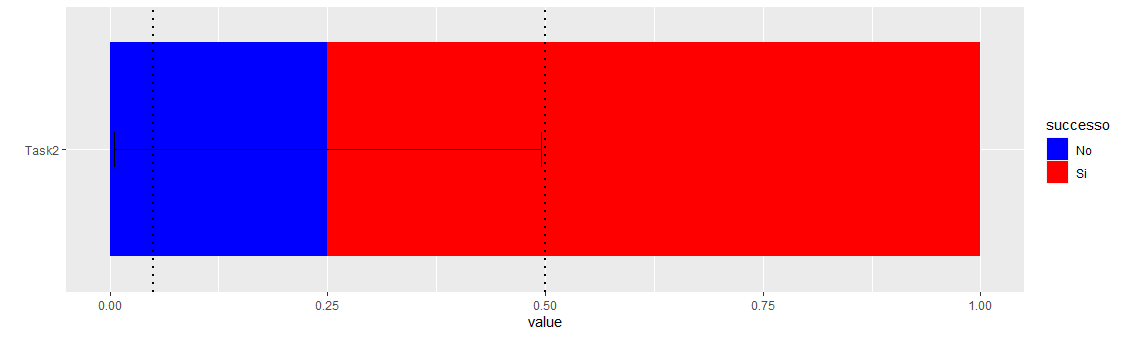
\includegraphics[scale = 0.45]{img/task/Dash2_TaskCalifornia_ErrorBar.png}
    \caption{Stacked bar chart task2}
\end{figure}

\subsection{Task terza dashboard}
Per l'ultima dashboard abbiamo sottoposto agli utenti tre diverse tipologie di task di difficoltà medio/facile:
\begin{itemize}
    \item Secondo te, in quale mese si è verificata la maggiore differenza percentuale?
    \item Quale ritieni che sia la percentuale di voli dirottati a dicembre?
    \item Secondo te, in che mese la percentuale di voli in orario è massima?
\end{itemize}
\begin{figure}[H]
	\begin{minipage}[b]{0.48\textwidth}
		\centering
		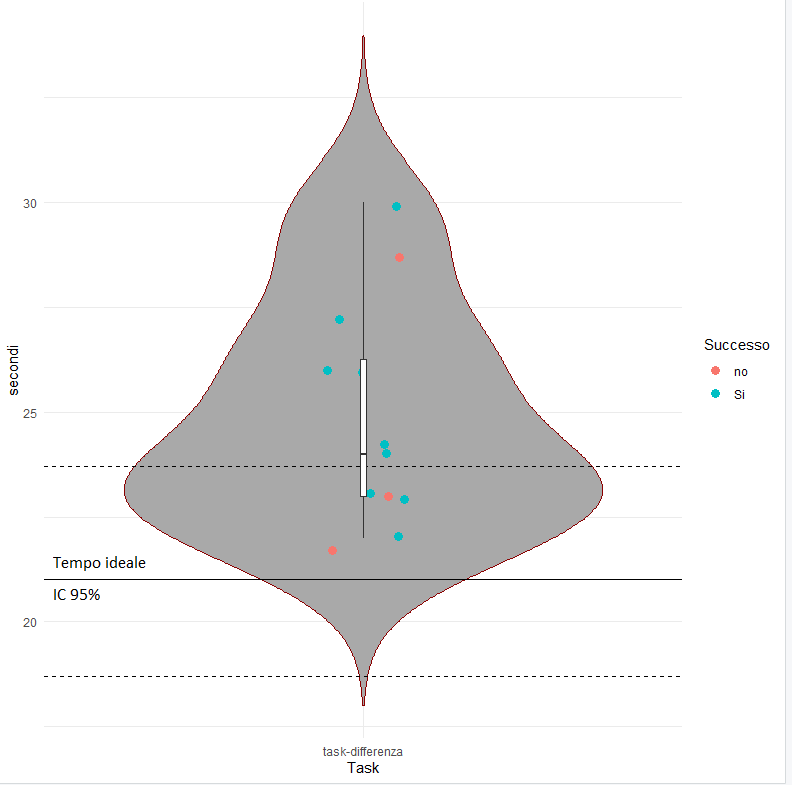
\includegraphics[width=\textwidth, height=7.5cm]{img/task/Dash3_TaskDifferenza.png}
        \caption{Task1 terza dashboard}
        \label{fig19}
	\end{minipage}
	\hfill
	\begin{minipage}[b]{0.48\textwidth}
		\centering
		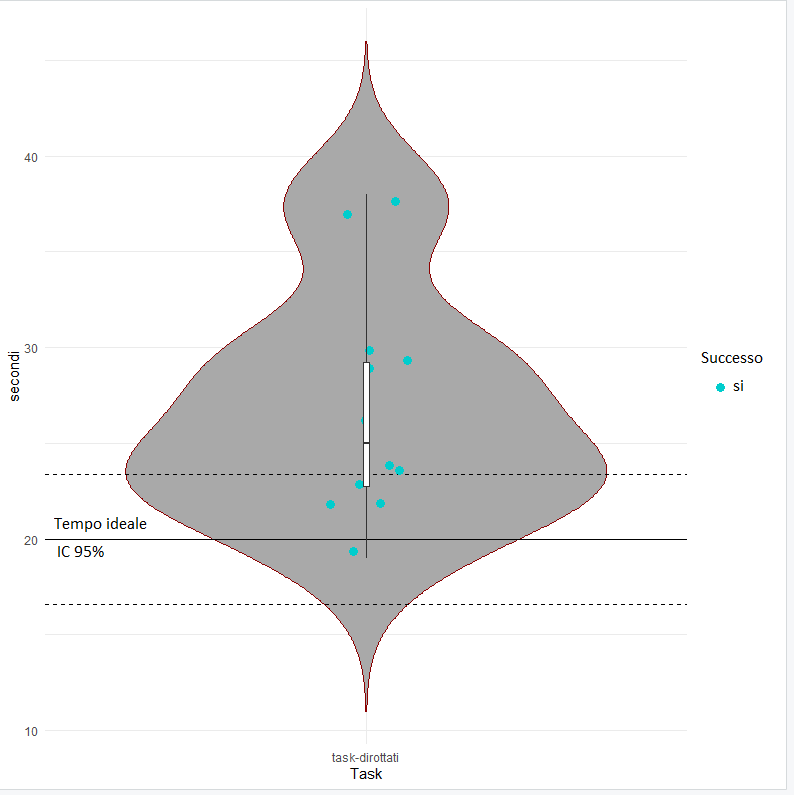
\includegraphics[width=\textwidth, height=7.5cm]{img/task/Dash3_TaskDirottati.png}
        \caption{Task2 terza dashboard}
        \label{fig20}
	\end{minipage}
\end{figure}
\begin{figure}[H]
    \centering
    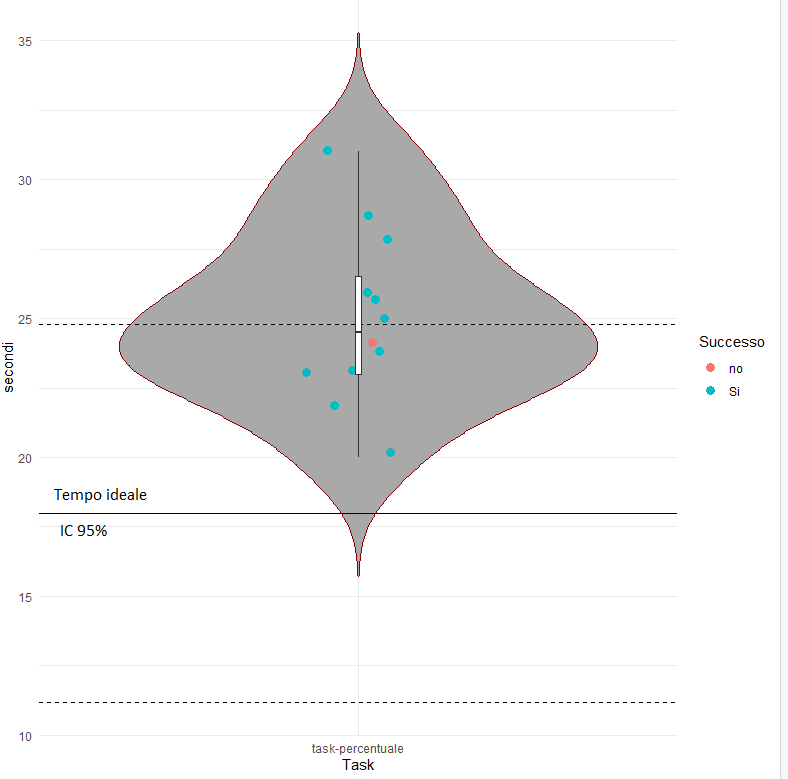
\includegraphics[scale = 0.5]{img/task/Dash3_TaskPercentuale.png}
    \caption{Task3 terza dashboard}
    \label{fig21}
\end{figure}
\noindent Il primo task, in figura \ref{fig19}, è quello che ha fatto registrare il maggior numero di errori 3, questi tre utenti hanno tutti risposto con la massima differenza percentuale positiva che si registra nel mese di novembre, il task però chiedeva di considerare anche i valori negativi. Il tempo medio di risposta per gli utenti è stato di quasi 25 secondi rispetto ai 21 secondi medi previsti, comunque sono individuabili anche alcuni outlier che potrebbero essere dovuti a scarsa dimestichezza dell'utente con la piattaforma o a lentezza nell'aggiornamento della pagina nel caso dei task interattivi.\\
Il secondo task, figura \ref{fig20}, è stato invece risolto con successo da tutti gli utenti probabilmente aiutati anche dall'indicazione, presente nella dashboard, che suggerisce agli utenti di cliccare sui nomi della legenda visualizzando così istantaneamente le percentuali per la categoria scelta.\\
Infine per l'ultimo task, figura \ref{fig21} si è registrato un solo errore, nonostante ciò il tempo medio necessario agli utenti per rispondere è abbastanza elevato. Probabilmente perché gli utenti hanno dovuto confrontare con precisione la percentuale nelle barre di settembre-ottobre-novembre in quanto la differenza tra questi mesi a livello percentuale era minima.\\
Si riportano di seguito gli stacked bar chart con la percentuale di risposte corrette ricevute per il primo e terzo task in quanto nel secondo non sono stati rilevati errori:
\begin{figure}[H]
    \centering
    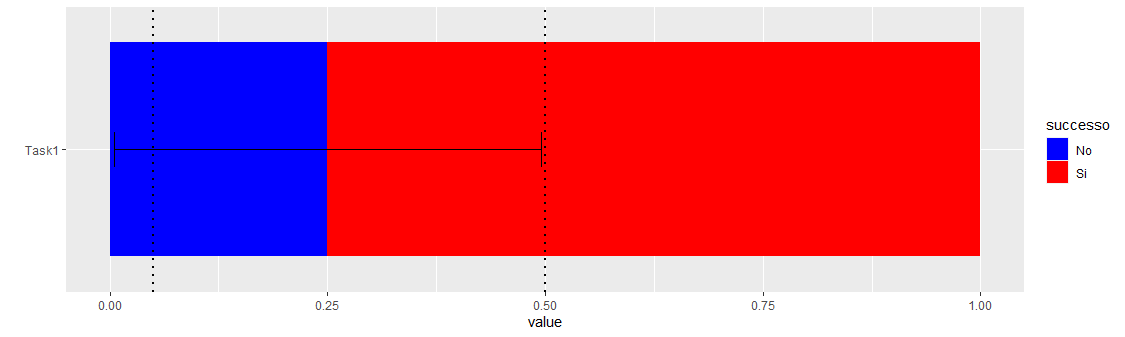
\includegraphics[scale = 0.45]{img/task/Dash3_TaskDifferenza_ErrorBar.png}
    \caption{Stacked bar chart task1}
\end{figure}
\begin{figure}[H]
    \centering
    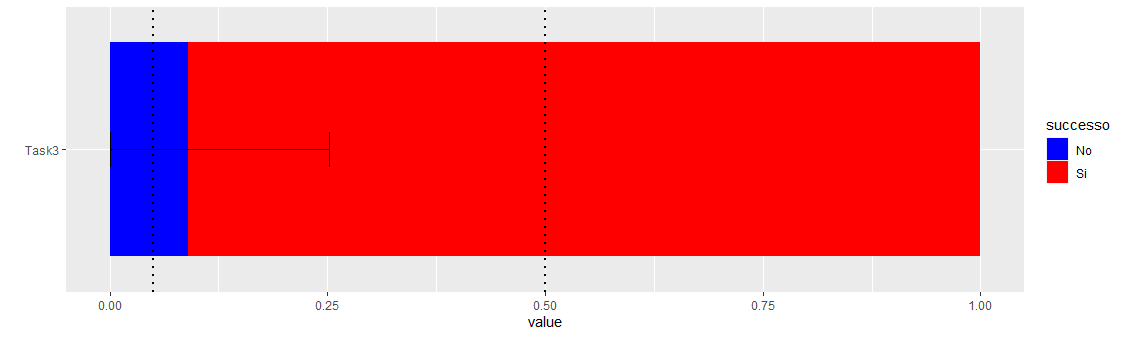
\includegraphics[scale = 0.45]{img/task/Dash3_TaskPercentuale_ErrorBar.png}
    \caption{Stacked bar chart task3}
\end{figure}

\section{Conclusione}
Grazie ai grafici realizzati è stato possibile rispondere alle domande prefissate, capendo, ad esempio, che il fatto di accumulare ritardo in partenza non sempre comporta un ritardo all'arrivo. Inoltre, si può notare che ci sono alcune compagnie aeree più performanti di altre in termini di ritardo negli anni in cui si ha fatto riferimento nell'analisi, anche se da un anno all'altro ci può essere una variazione notevole. E che addirittura ci sono alcune eccezioni che riescono mediamente ad arrivare a destinazione in anticipo. Tra queste, però, non figurano le 4 compagnie statunitensi principali, delle quali la Delta Airlines risulterebbe essere quella che accumula meno ritardo all'arrivo.
Comunque, da un punto di vista globale, si evince che i mesi estivi, ma anche per i periodi festivi di dicembre e gennaio o giorni come il lunedì, sono caratterizzati generalmente dai ritardi più consistenti. Alla base, probabilmente, contribuirebbero in negativo una serie di fattori come l'elevato numero di viaggiatori, fenomeni meteorologici avversi e il personale sotto stress. Ciò, tuttavia, sembra essere trascurabile nei mesi di marzo e settembre,  ma anche per il giovedì, dove i ritardi diminuiscono nettamente.\\
Ad ogni modo, il calo delle performance sembra essere associabile anche alle aree più densamente popolate degli Stati Uniti. Forse perché banalmente essendoci un traffico aereo maggiore, la probabilità di registrare ritardi chiaramente è notevole.\\
Infine, è stato possibile osservare anche che i voli cancellati, che sono sempre molto meno rari di quelli dirottati, si concentrano tendenzialmente nei mesi invernali climaticamente sfavorevoli, soprattutto nel 2019 a causa dell'intensa ondata di freddo registrata in un' ampia area degli Stati Uniti.\\
In aggiunta, passando a considerazioni qualitative sul lavoro svolto, grazie alle valutazioni e ai task svolti dagli utenti, è emerso che le infografiche realizzate vengono solitamente ritenute informative e chiare anche se non particolarmente belle e intuitive, nonostante poi la valutazione complessiva sia sempre più che discreta. Probabilmente la poca intuitività riscontrata ha influito sui tempi di risposta ai task da parte degli utenti che si sono rivelati essere quasi sempre superiori al tempo ideale.







\newpage
\section{Link alle visualizzazioni}
Si riportano i link per visualizzare ed interagire con le visualizzazioni create.\smallskip\\
\textbf{Prima dashboard} \url{https://public.tableau.com/profile/silvia6565#!/vizhome/Progetto_Airline_On_Time_Performance_storia/Dashboard1}\smallskip\\
\textbf{Seconda dashboard} \url{https://public.tableau.com/profile/silvia6565#!/vizhome/Progetto_Airline_On_Time_Performance_storia/Dashboard2}\smallskip\\
\textbf{Terza dashboard} \url{https://public.tableau.com/profile/silvia6565#!/vizhome/Progetto_Airline_On_Time_Performance_storia/Dashboard3}\smallskip\\
\textbf{Storia} \url{https://public.tableau.com/profile/silvia6565#!/vizhome/Progetto_Airline_On_Time_Performance_storia/Storia}

\newpage
\section{Bibliografia}
\nocite{*}
\printbibliography[heading=none] %Prints the entire bibliography


\end{document}